\documentclass{article}

\usepackage[utf8]{inputenc}
\usepackage{graphicx}
\usepackage{float}
\usepackage{csquotes}
\usepackage{hyperref}
\usepackage{amsmath}
\usepackage{amsfonts}
\usepackage{enumerate}
\usepackage{dirtytalk}
\usepackage{lineno}
\usepackage{authblk}

\let\up\textsuperscript
\title{Escaping optimization traps: The role of cultural adaptation and cultural exaptation in facilitating open-ended cumulative dynamics} 

\author[1]{James Winters\thanks{winters@shh.mpg.de}}
\affil[1]{Max Planck Institute for the Science of Human History, Germany}

\begin{document}

\maketitle

\begin{abstract}
    \noindent Explaining the origins of cumulative culture, and how it is maintained over long timescales, constitutes a fundamental challenge for theories of cultural evolution. Previous theoretical work has emphasised two fundamental causal processes: cultural adaptation (where technologies are refined towards a functional objective) and cultural exaptation (the repurposing of existing technologies towards a new functional goal). Yet, despite the prominence of cultural exaptation in theoretical explanations, this process is often absent from models and experiments of cumulative culture. Using an agent-based model, where agents attempt to solve problems in a high-dimensional problem space, the current paper investigates the relationship between cultural adaptation and cultural exaptation and produces three major findings. First, cultural dynamics often end up in {\em optimization traps}: here, selection for optimized solutions cause the dynamics of change to cease, with populations entering a state of equilibrium. Second, escaping these optimization traps requires cultural dynamics to explore the problem space rapidly enough to create a moving target for optimization. This results in a positive feedback loop where there is an open-ended growth in both the diversity and complexity of cultural solutions. Finally, the results helped delineate the roles played by social and asocial mechanisms, with asocial mechanisms of innovation driving the emergence of cumulative culture and social mechanisms of within-group transmission helping maintain these dynamics over long timescales.
\end{abstract}

\section{Introduction}
Humans are prodigious problem solvers. Unlike many non-human animals, humans seem particularly adept at incrementally discovering and exploiting solutions with higher payoffs~\cite{tennie_claudio_ratcheting_2009,acerbi_alberto_social_nodate}, as evident in the bewildering growth of technological sophistication over the last several thousand years. Access to increasingly complex solutions allowed human groups to enter into and thrive across a variety niches via cultural as opposed to biological adaptations~\cite{richerson_not_2008,henrich_secret_2015,laland_darwins_2018}. No better is this illustrated than in our use of clothing and weapons as technological solutions for environmental challenges. While polar bears evolved thick layers of blubber, large paws, and specialised carnassials to survive and hunt in Arctic environments, the Inuit achieved comparable outcomes by modifying and extending existing technologies to invent parkas, mukluks, and harpoons.

These distinct advantages are often attributed to the ability of cultural evolutionary dynamics to facilitate a cumulative process: here, solutions with higher payoffs do not need to be independently rediscovered, but can instead be transmitted from individual-to-individual via social learning mechanisms~\cite{boyd_culture_1988,dean2014human,mesoudi_alex_what_2018}. Whilst non-human animals have culture~\cite{kawamura1959process, whiten1999cultures, hunt2004direct, krutzen2005cultural}, and exhibit a high level of cognitive and behavioural sophistication~\cite{emery2004mentality,penn2007causal,piantadosi2017true}, humans are alone in their capacity to modify these traits in a direction of open-ended complexity~\cite{Heyes_1993, tomasello_kruger_ratner_1993, boyd1996culture} (see \cite{mesoudi_alex_what_2018} for a recent overview). As with biological evolution, this cumulative process provides a powerful explanation for the fit between technological solutions and ecological problems via {\em cultural adaptation}: by generating different solutions for a given problem, a population can gradually select from this pool of variation and move closer to an optimal solution~\cite{boyd_culture_1988,boyd_why_1995,enquist_critical_2007,richerson_not_2008,henrich_secret_2015,laland_darwins_2018}.

Less attention has been paid to another prominent process in the evolution of technology: {\em cultural exaptation}~\cite{kauffman_origins_1993,mokyr1998induced,arthur2009nature,johnson2011good,solee2013evolutionary,andriani2013exaptation}. Initially coined by Gould \& Vrba~\cite{gould1982exaptation}, although the concept itself dates back to Darwin~\cite{darwin2004origin} in biology ({\em preadaptation}) and to Schumpeter~\cite{schumpeter1939business} in economics, exaptation is when a biological or cultural trait originally adapted for use in one functional role is co-opted and repurposed towards a new function. Whereas cultural adaptation follows from a search over the pool of possible solutions, cultural exaptation inverts the causality of this process: it searches the space of possible problems in an effort to find a novel problem for a given solution. Viagra, for instance, was originally invented as a potential solution for angina, but during clinical trials it was discovered to be a far more effective remedy for erectile dysfunction~\cite{andriani2015measuring}. The history of technology is replete with similar instances: from Gutenberg co-opting the screw-driven wine press in the creation of the printing press~\cite{solee2013evolutionary} to the re-purposing of iron door hinges as ship rudders~\cite{boyd2013cultural} or the discovery that processing biological hazards can be done via the high temperatures required for vitrification~\cite{dew2004economic}.

How do these two processes of cultural adaptation and cultural exaptation interact to shape and constrain cultural evolutionary dynamics? In biological evolution, Darwin envisaged adaptation and exaptation as part of a cycle of open-ended novelty and refinement: it is a process of taking an already adapted trait, repurposing it for a new function, and then adaptively tuning this trait for its new functional role via natural selection. An oft-cited example is the repurposing of feathers, which were originally used for thermoregulation, as a means of facilitating flight~\cite{gould1982exaptation}. Theoretical frameworks in cultural evolution have also recognised the importance of exaptation in the domains of technology~\cite{boyd2013cultural} and language~\cite{lass1990things}. Yet, despite the prominence of cultural exaptation in these frameworks, this process is curiously absent from models and experiments into cumulative culture~\cite{mesoudi_alex_what_2018}.

One reason for this omission is the focus on specific types of cumulative culture. Debates over what constitutes cumulative culture, as well as questions over its presence in non-human animals, is the source of much consternation (for recent reviews, see~\cite{miton2018cumulative,mesoudi_alex_what_2018}). Social transmission experiments, for instance, tend to investigate processes of functional refinement. In these cases, the dynamics of change are more akin to a {\em cumulative optimization} process, whereby an experimental population moves closer to an optimal solution within the bounds of its input problem(s) and the available resources. An example of this is found in a recent experimental study of pigeon flight path optimization~\cite{sasaki_cumulative_2017}: here, pigeons are only able to discover the quickest route when information about flight routes are socially transmitted. Similar experiments with human participants, such as transmission chains of paper aeroplanes~\cite{xxxx}, spaghetti towers~\cite{xxxx}, and fishing nets~\cite{caldwell2016experimental}, all reach comparable outcomes.

As others have suggested~\cite{mesoudi_alex_what_2018}, cumulative optimization in this sense qualifies as an instance of cumulative culture, but it is insufficient to produce the open-ended dynamics inherent to human cultural domains (such as technological evolution). Pigeons do not apply insights from the optimization of flight paths to other domains and the cumulative dynamics only persist until an optimal flight path is reached (a fact recognised by~\cite{sasaki_cumulative_2017}). The only available options in such instances are to remain in the current state or transition to a less-optimal configuration. In essence, populations become stuck in an optimization trap where the dynamics of change cease and enter a state of equilibrium. By contrast, inventions such as writing or the steam engine are capable of changing the bounds within which cultural dynamics operate, introducing populations to novel problems as well as allowing them to more readily generate novel solutions.

Much of the emphasis in computational models is on the open-endedness of cumulative culture. In recent models, this often corresponds to cumulative growth in either the diversity~\cite{mesoudi2011variable,kolodny2015evolution,creanza2017greater} or complexity~\cite{enquist2011modelling,lewis2012transmission,derex2018divide} of cultural traits. In many ways, these models suffer from the opposite problem to that found in experiments: the absence of any overt functional target. Functional constraints are often not explicitly modelled or they form a single fitness proxy. Generally, in cases where fitness is modelled, fitness is assumed to be an intrinsic feature of a cultural trait (e.g., via a utility function~\cite{lewis2012transmission}) and there is no notion of how different functional constraints shape the evolution of these traits. While this simplifying assumption proves useful in many circumstances, it overlooks the role played by functional constraints and marginalises the contributions of cultural exaptation in driving open-ended cumulative culture.

Computationally-inspired theories offer a promising avenue for addressing such issues by modelling cultural dynamics as search processes over solution {\em and} problem spaces. In the next section, a computational framework of cultural evolution is outlined, and used to demonstrate that high-dimensional problem spaces introduce constraints rarely considered in standard cultural evolutionary approaches. Then, using an agent-based model where agents attempt to solve problems in this high-dimensional problem space, the current paper investigates the relationship between cultural adaptation and cultural exaptation in shaping cultural evolutionary dynamics. Two general parameters, corresponding to the extent to which solutions undergo optimization ($\lambda$) and the rate with which agents explore the problem space ($\Theta$), are manipulated. Four important findings follow from the inclusion of a high-dimensional problem space:

\begin{enumerate}[(i)]
    \item Strong optimization pushes populations into optimization traps with low complexity solutions;
    \sloppy
    \item Escaping these optimization traps requires increasingly high rates of exploration-driven exaptation relative to the strength of optimization;
    \item The emergence of open-ended cumulative dynamics relies on high rates of innovation relative to within-group transmission;
    \item However, as solutions grow in complexity and problems become more difficult to solve, the selection of socially transmitted solutions plays an increasingly prominent role in maintaining this open-ended cumulative dynamic.
\end{enumerate}

\section{Model}
\sloppy
Approaching cultural evolutionary dynamics in this model starts from the premise that cultural information is {\em algorithmic}. Algorithm is referred to in a general sense to mean a procedure or recipe that consists of an input problem (which may be empty) and an organised series of steps that results in a solution~\cite{xxxx,mayfield2013engine}. Computer programs are algorithmic because they provide a set of specific instructions for transforming a given input into an output that can then be stored. Sorting algorithms, for instance, take a list of randomly ordered elements and transform this into a new sequence based on some predefined order (such as numerical or lexicographic). Similarly, cultural information stored in recipes, grammars, and motor sequences are algorithmic; a set of mental instructions can be used to create tomato soup, learn a language, and produce Oldowan flakes~\cite{arthur2009nature,charbonneau_all_2015,xxxx}.

In this sense, cultural information exists as generative procedures inside the minds of individuals, and is manifest in populations as observable behaviours or tangible artefacts~\cite{ferdinand2015inductive}. Thinking of cultural information as algorithmic allows us to formulate constraints on cultural evolutionary dynamics in terms of solutions and input problems. Solutions exist as the physical manifestations of culture and input problems are the specific functional challenges. Cultural evolutionary dynamics can therefore be modelled as a process of searching and sampling both the space of solutions and problems. If a search process is biased to find solutions that better approximate a given input problem, then we can think of this optimization process as cultural adaptation. Alternatively, if the search process seeks out novel input problems for a specific solution, then this process of re-purposing solutions is a form of cultural exaptation.

To capture these processes, solutions and problems are represented as binary strings of $n$-length. Modelling solutions and problems in this way affords (potentially) unbounded searches over solution and problem spaces. All model runs took place over a $100$ generations and every generation comprised of $10$ time steps. A single run was initialised with a fixed population of agents ($N=100$) who were randomly assigned to input problems of length $\ell(p)=2$ and provided with randomly generated starting algorithms that produced solutions in the range $\ell(s)=[2,4]$. At each time step, an agent generates a pool of possible solutions from asocial and social sources (see section~\ref{xxxx}). On the basis of the optimization strength ($\lambda$), as well as the current input problem, one of these solutions is then adopted and assigned to an agent's memory as their stored solution (see section~\ref{xxxx}). The exploration threshold ($\Theta$) interacts with the current fit between a solution and an input problem to determine whether or not an agent moves to a new problem (see section~\ref{xxxx}). Following 10 time steps, an agent dies and their currently stored solution is inherited by a newly created offspring agent (see section~\ref{xxxx}).

%Which of these solutions an agent adopts is influenced by the current input problem and how it interacts with a parameter controlling the strength of optimization ($\lambda$) (see section~\ref{xxxx}). A second parameter governing the exploration threshold ($\Theta$) then determines whether or not an agent moves to new problem on the basis of the fit between a solution and the current input problem (see section~\ref{xxxx}).

\begin{figure}[H]
\begin{center}
    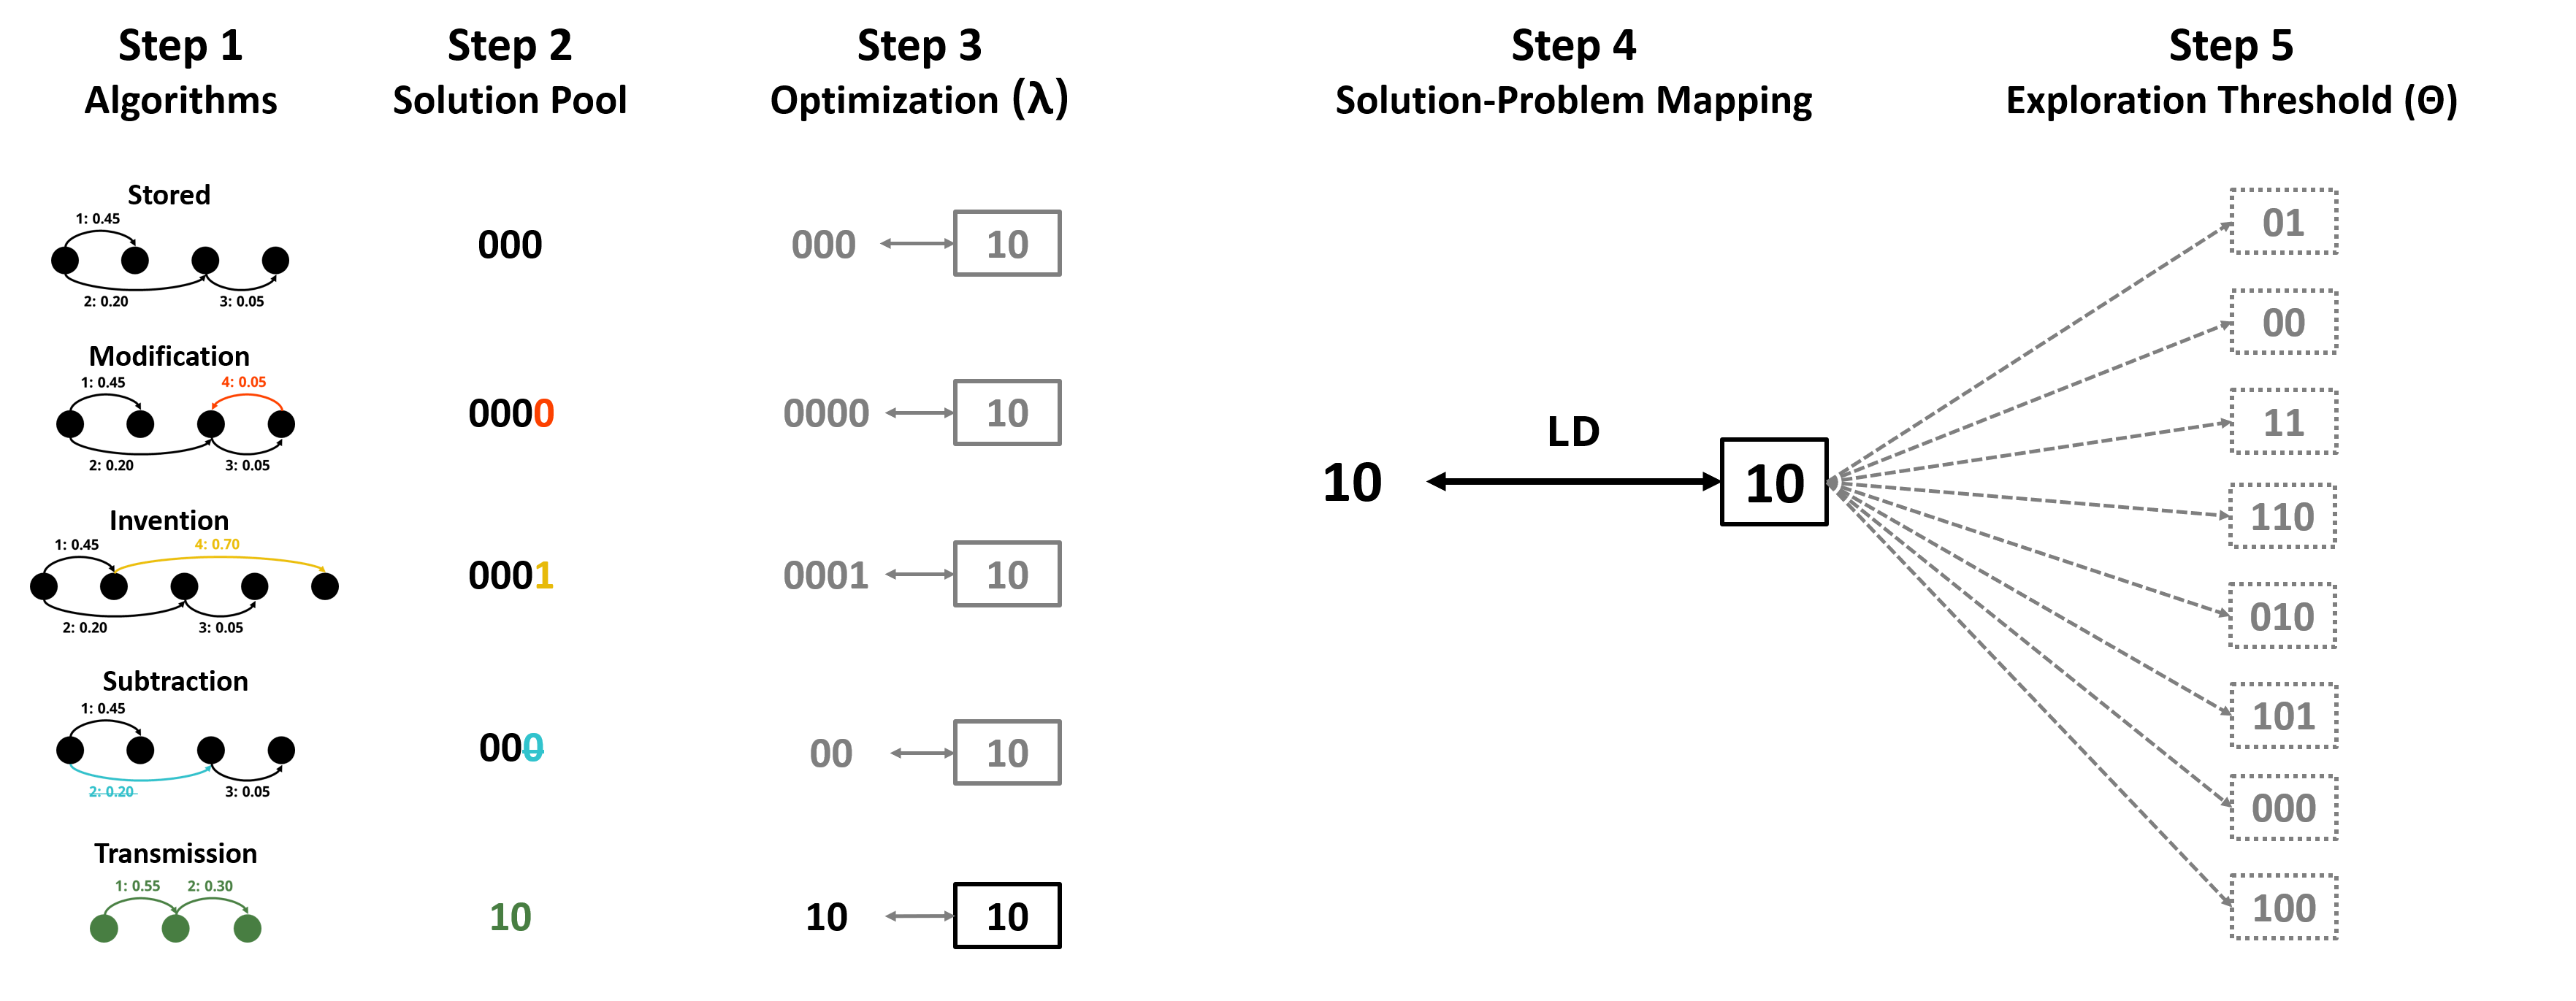
\includegraphics[width=\linewidth]{mechanisms.png}
\end{center}
    \caption{The process an individual agent performs within a single time-step. \textbf{Step 1:} Agents use a series of mechanisms to indirectly alter a bit string via a graph. The stored algorithm refers to the graph that currently occupies an agent's memory (as determined by the previous time step). This stored algorithm is acted upon by three asocial mechanisms of modification, invention, and subtraction. Asocial mechanisms can only make single modifications per time-step. Transmission is when an agent receives an algorithm from another agent within the population. \textbf{Step 2:} Each of these mechanisms generate a pool of solutions by translating the algorithm into a bit string (i.e., a solution). \textbf{Step 3:} Which of these solutions is adopted depends on whether optimization is biased or stochastic (as determined by $\lambda$). If optimization is biased, an agent compares each solution to their input problem and chooses the one with the best fit (otherwise, if the choice is stochastic, then a solution is randomly chosen from the pool). \textbf{Step 4:} An agent uses their current solution-problem mapping to motivate whether or not they consider a novel problem (as determined by the exploration threshold $\Theta$). \textbf{Step 5:} This movement is restricted to local problems (i.e., those that differ from the current input problem by single-edit substitutions).}
    \label{fig:mechanisms}
\end{figure}

\subsection{Cultural adaptation}
Input problems are a key biasing factor in determining the trajectory of cultural evolutionary dynamics via cultural adaptation: a search optimization process over the space of solutions that results in an improved fit between a solution and an input problem. Limitations on the design of a solution exist in the form of functional constraints, i.e., how well adapted a solution is at solving a problem. This refers to the specification of the input problem (building a handaxe for cutting meat) and the ways in which it constrains the possible outcomes by creating an adaptive target (useful meat cutting solutions need to induce a certain level of sheer stress). Cultural adaptation is modelled here as a process of improving the fit between an input problem and a solution string. The Levenshtein distance (LD) allows us to formally measure this fit:

\begin{equation} 
LD_{s,p} (i,j) =
\begin{cases}
    max(i,j) & \text{if $min(i,j)=0$}, \\
    min \begin{cases}
    LD_{s,p}(i - 1,j) + 1 \\
    LD_{s,p}(i, j - 1) + 1 \\
    LD_{s,p}(i - 1,j - 1) + 1_{s_i \neq b_j} \\
    \end{cases}
    & otherwise.
\end{cases}
\end{equation}

where $LD_{s,p} (i,j)$ is the distance between the $i$th element of solution $s$ and the $j$th element of problem $p$. As such, the Levenshtein distance between two strings tells us the minimum number of singe-element edits (insertions, deletions or substitutions) required to transform one string into the other. Fewer transformations between a problem and a solution acts as a proxy for the level of optimization. Solution-problem mappings with high a LD are less optimized than those with lower values. A fully optimized solution therefore corresponds to $\min_{s,p} LD(s,p)=0.0$ as a solution and its input problem are identical. 

Facilitating this search are three general processes corresponding to the {\em generation}, {\em transmission}, and {\em optimization} of solutions.

\subsubsection{Solutions}
Solutions in this model represent technological artefacts and are generated using directed graphs (for a similar approach, see~\cite{enquist2011modelling}). This approximates two features of technological solutions: the cultural artefact (a bit string) and the underlying algorithm (a graph). Graphs were initially constrained so that agents start with solutions of lengths $\ell(s)=[2,3,4]$. Formally, a graph $G$ consists of a triple $(V,E,\Omega)$ where $V$ is the set of nodes $v \in V$, $E$ is the set of edges $e \in E$, and $\Omega$ is a function mapping every edge to an ordered set of values $\Omega: E \to \mathbb{N}$. Each node comprises of a value in the interval $[0,1]$ and each edge is assigned a bit of either $0$ or $1$. A single bit is derived from the average of two nodes that are connected via an edge and rounded the nearest integer. As edges are directed, any node can connect to another node within $V$. Two exceptions are no loops (i.e., nodes that connect to themselves) and no duplicate edges (i.e., a directed connection can only exist once). $\Omega$ arranges the set of edges to produce the bit string (the solution) and is determined by an ordinal value.

\begin{figure}[H]
\begin{center}
    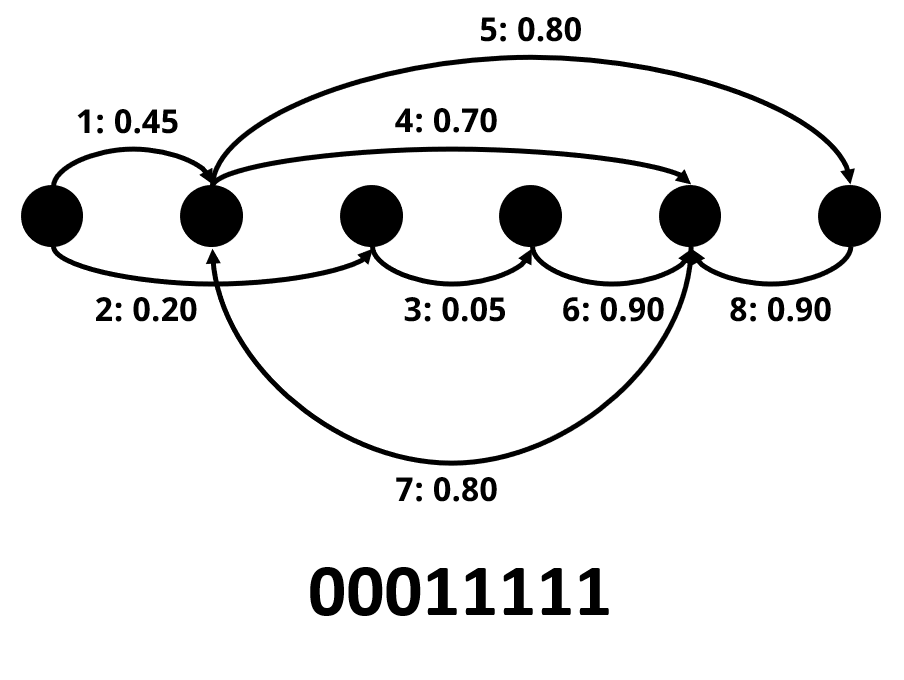
\includegraphics[width=\linewidth]{algorithm.png}
\end{center}
    \caption{An example of cultural algorithm. Black circles represent nodes and the arrows connecting nodes represent directed edges. Each edge has a pair of numbers: the first denotes the order of that edge in the set and the second corresponds to the value of that edge. An edge value is the average of its two nodes. This value is rounded to the nearest integer (either $0$ or $1$) to produce a single bit. Edge order is an ordinal value that represents the position of a bit in a solution string.}
    \label{fig:algorithm}
\end{figure}

\subsubsection{Asocial generative mechanisms}
Generating solutions refers to the introduction of novelty and diversity into a population via asocial mechanisms. In this model, changes to a solution are done indirectly via the graph-based procedure, with agents having access to three general mechanisms for innovating (see Fig.~\ref{fig:mechanisms}):

\begin{itemize}
    \item {\em Invention} introduces a new bit by creating and then connecting a new node to an existing one. New nodes are assigned a randomly generated value in the range $[0,1]$.
    \item {\em Modification} changes a pre-existing solution by connecting two existing nodes to form a new edge. 
    \item {\em Subtraction} shortens a bit string by randomly removing an existing edge and ensures that innovation is not unidirectional.
\end{itemize}

A general assumption is that these generative mechanisms are restricted: Agents can only create or remove a single bit. Imposing such limitations approximates the idea that innovations are often introduced via limited experimentation within a restricted search space. Discovering some solutions are easier than others because they require less time and resources to produce (given a starting state). Similar notions are present in Tennie and colleagues' {\em Zone of Latent Solutions}~\cite{tennie_claudio_ratcheting_2009}: here, solutions that are reachable via asocial means have a high probability of being independently (re-)invented.

\subsubsection{Social transmission mechanisms}
Transmission is the movement of information between individuals and corresponds to how individuals learn from others via observation and teaching~\cite{gergely2006sylvia}. Two types of social transmission are present in this model: a vertical transmission process of {\em inheritance} and a {\em within-group} process of horizontal transmission. Vertical transmission happens at each generation (every $10$ time-steps) and takes place between a parent agent (who dies) and a newly created child agent. The choice of $10$ time-steps is arbitrary, but it does capture the finite lifetimes of individuals and recognises that the contributions of a single individual are generally circumscribed when considering long timescales. As the name suggests, within-group transmission takes place between individuals at a given generation, and involves one agent learning a cultural algorithm from another randomly selected agent within the population.

Both forms of transmission are indirect (agents transmit algorithms, not solutions), reconstructive (solutions are generated using the underlying algorithm), and biased (reconstructions are biased towards efficient representations). This aligns with the general idea that transmission is an inductive process guided by both the input data and the prior cognitive biases of learners~\cite{chater2003simplicity,griffiths2007language,kirby2007innateness,culbertson2016simplicity}. Transmitting an algorithm is thus analogous to learning a recipe or procedure and is instantiated here as a process of reconstructing the shortest path between nodes. Dijkstra's algorithm is used to construct a graph distance matrix $\bigl(d_{i \  j}\bigr)$ that computes all distances from $v_i$ to node $v_j$. The shortest path is one which visits all connected nodes in the shortest number of steps. This assumes graphs are directed with equally weighted edges and that the starting point is the first node in the graph (as determined by $\Omega$, see section~\ref{xxxx}).

\subsubsection{Strength of optimization ($\lambda$)}
Optimization is modelled as an individual-level decision making process over the pool of solutions derived from social and asocial sources. The goal being for agents is to find a solution that improves the fit with the current input problem. One advantage of the approach used here is that it explicitly builds a bridge between individual-level processes and population-level outcomes~\cite{derex2018divide}. This presents a notable departure from some recent cultural evolutionary models of cumulative culture in which individual-level processes are ignored in favour of solely focusing on the population-level distribution of cultural traits~\cite{enquist2011modelling,lewis2012transmission}.

Manipulating the strength of optimization ($\lambda$) allows us to directly investigate the extent to which this decision-making process is biased or stochastic. The current model examined the following parameter values for $\lambda$: $[0.0,0.2,0.5,0.8,1.0]$. When the strength of optimization is at maximum ($\lambda=1.0$), agents choose a solution based solely on its ability to optimally solve the current input problem. The pool from which these solutions are chosen is restricted to the currently stored solution and variants generated via asocial or social means. A maximally biased choice is one where an agent compares the Levenshtein distance of an input problem ($p$) with each solution ($s$) in the pool $X$ and selecting the most optimized one:

$$\min\limits_{s \in X} LD(s,p)$$

As the strength of optimization is decreased, stochastic factors play an increasingly prominent role in determining which solution is or is not adopted. If the strength of optimization is $\lambda=0.0$, the process of choosing solutions is purely stochastic, i.e., there is no preference for solutions based on the Levenshtein distance, whereas a $\lambda=0.8$ means that on average $80\%$ of agent's productions will be biased and $20\%$ will be stochastic. 

\subsubsection{Solution Complexity $H_{L}(S)$}
Solution complexity is measured as the product of Shannon Entropy~\cite{shannon1949mathematical,cover2012elements} and the length of a solution: 

\begin{equation}
H_{L}(S) = -\sum_{n=1}^{n} P(S_i) \ log_2 P(S_i) \ \ell(S)
\end{equation}

where $S_i$ is a binary value found within a solution, $P(S_i)$ is the probability of value $i$ given a solution string $S$, and $\ell(S)$ is the length of the solution. $H_{L}(S)$ is therefore the average amount of information within a specific solution string of $N$-length. In this sense, $H_{L}(S)$ acts as a proxy for solution complexity: lower $H_{L}(S)$ strings are less complex than ones with a higher $H_{L}(S)$. 

This assumes complex solutions are longer strings where the distribution of bits is close to uniform (i.e., $1$ bit) and provides a relatively simple way of capturing simple solutions (i.e., those that are closer to $0$ bit). However, a well-recognised limitation of this approach is that it fails to discriminate between strings of equal length, where one forms a highly ordered sequence (e.g., $01010101$ or $00001111$) and the other approximates an algorithmically irregular sequence (e.g., $01101001$).

\subsection{Cultural exaptation}
Cultural exaptation was defined earlier as a process where solutions used for one problem are repurposed to solve a novel problem. It was also argued that this can be framed as a search process over the space of possible problems. One recurrent observation is that exaptation normally occurs in domains where there are functional overlaps between the original and novel input problems~\cite{arthur2009nature,mastrogiorgio2016innovation}. Co-opting technology in such a way also implies that repurposed solutions are to some extent optimized for solving their original input problem. In some sense, Viagra was well-designed for the purpose of inducing vasodilation; it just happened to be better suited for encouraging blood flow to certain regions as opposed to others.

\begin{figure}[H]
\begin{center}
    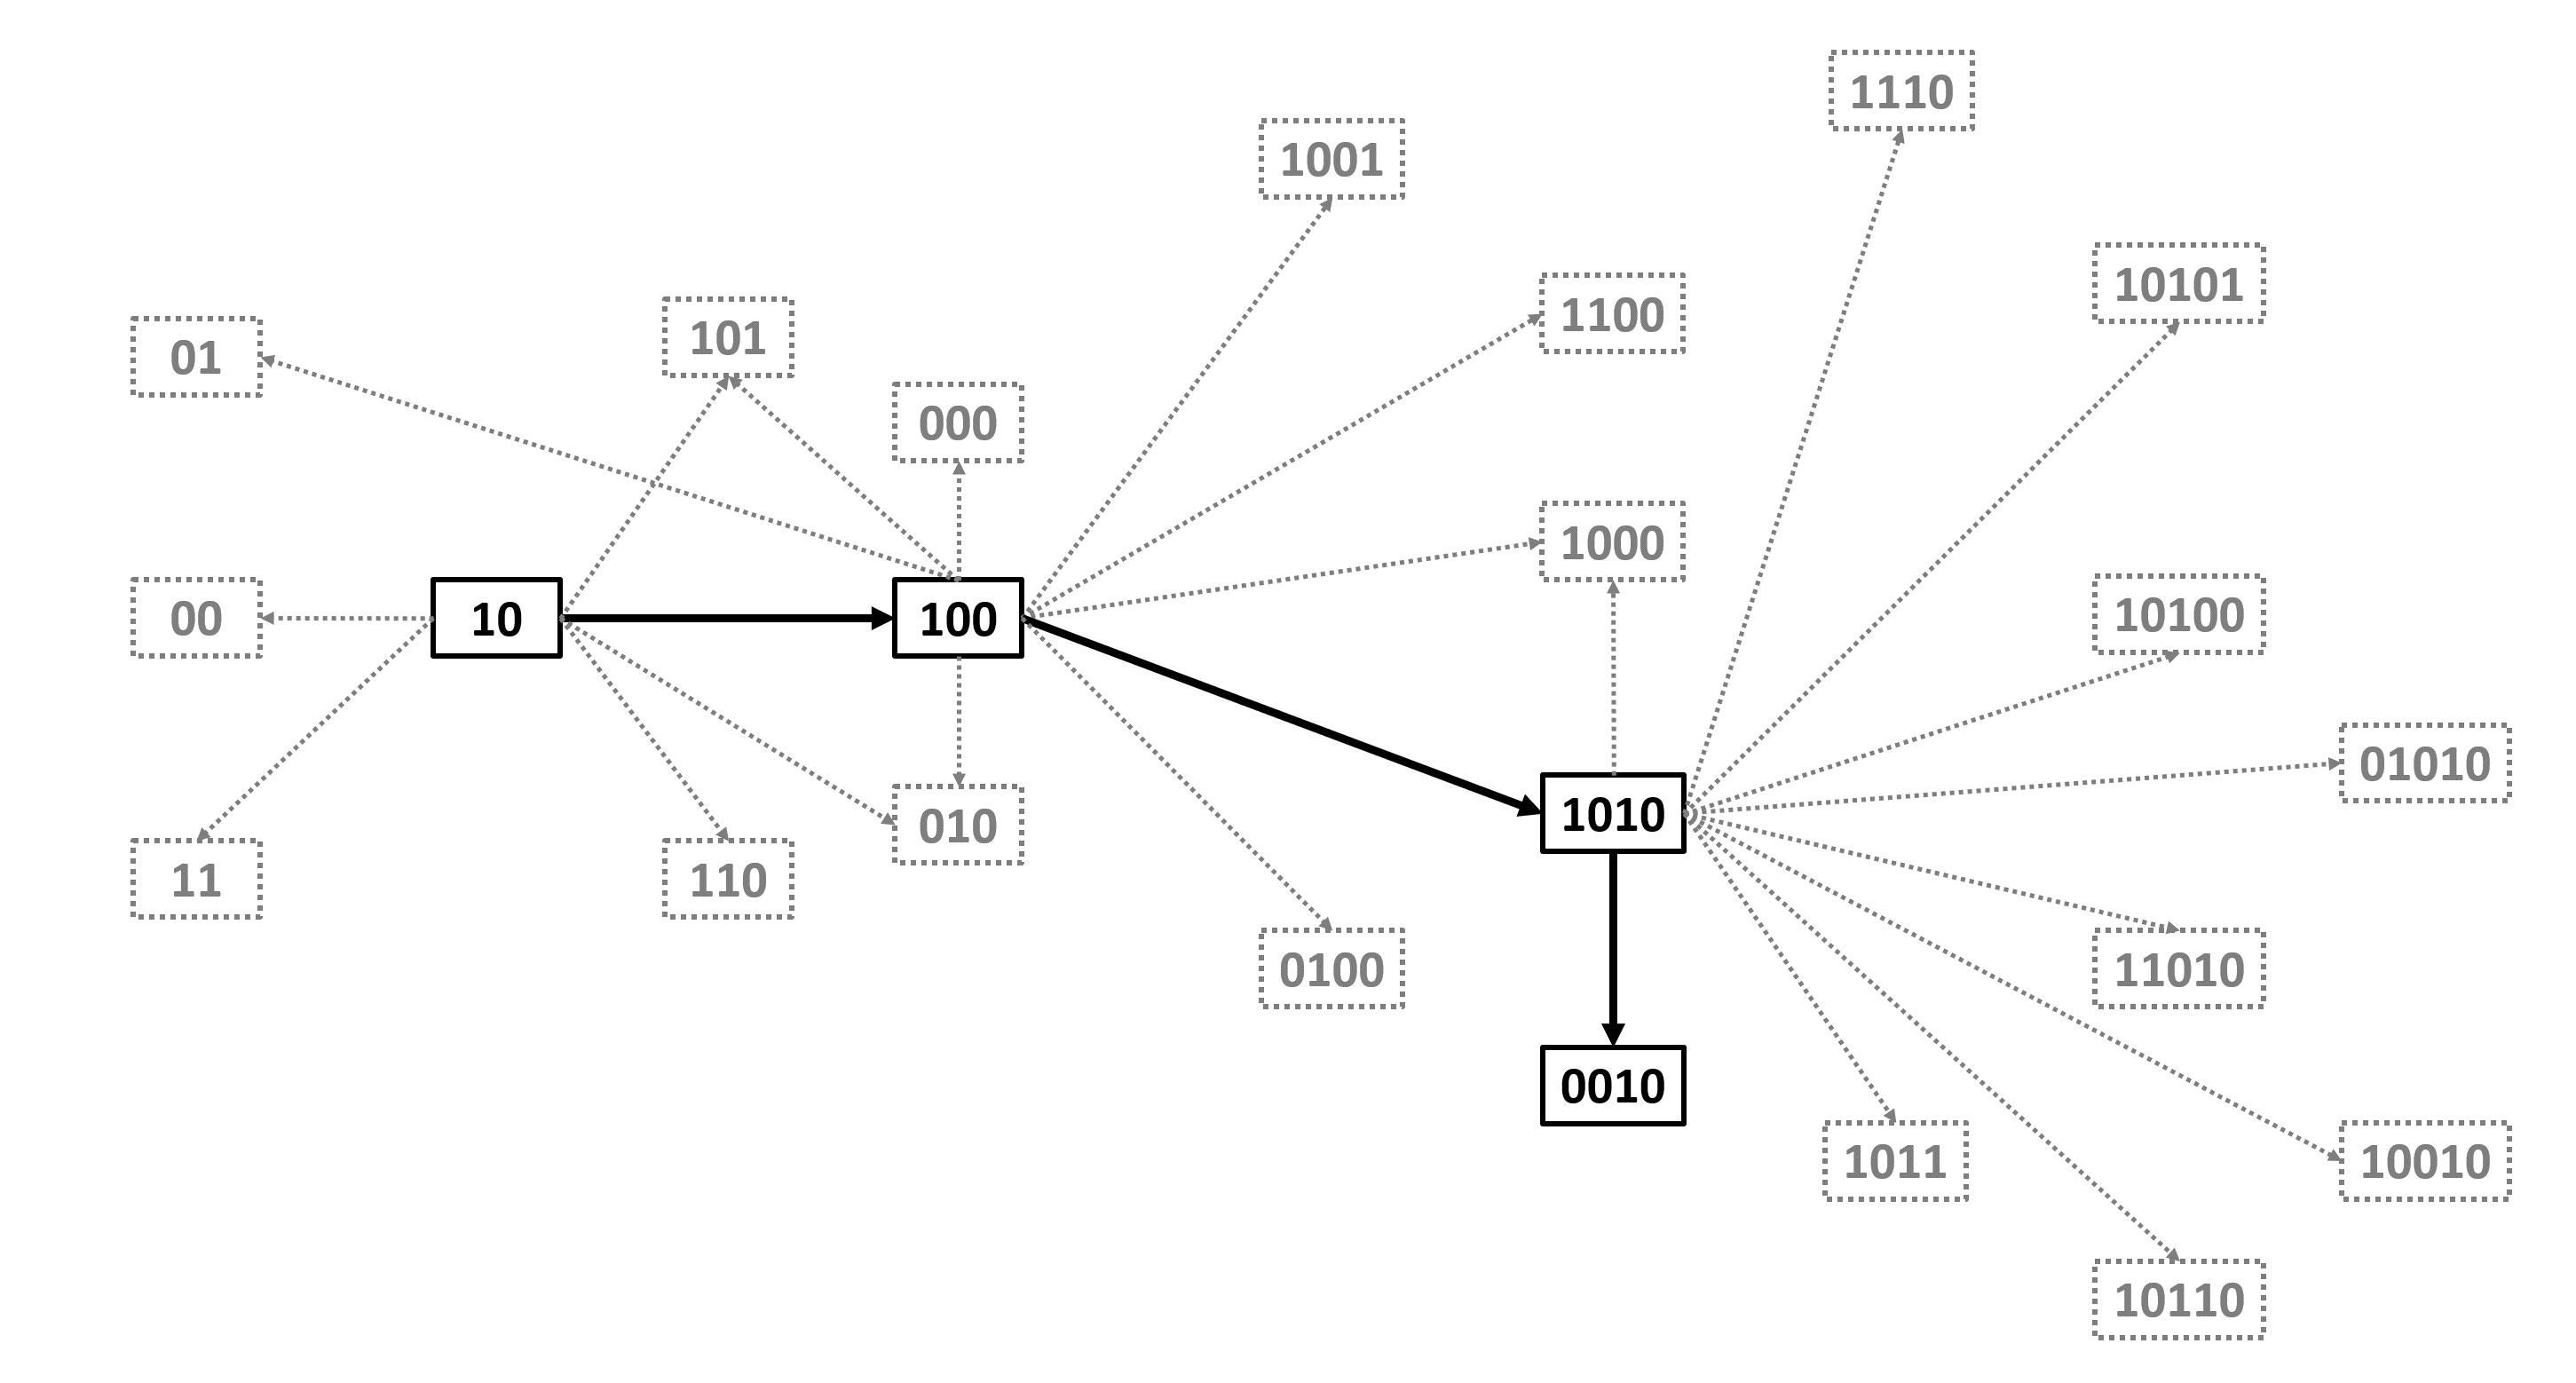
\includegraphics[width=\linewidth]{probspace.png}
\end{center}
    \caption{XXXX.}
    \label{fig:topology}
\end{figure}


Introducing a high-dimensional problem space is required if we are to simulate the process of cultural exaptation as a search process over the space of problems. The problem space here forms a connected graph consisting of all possible permutations of an $N$-length binary string. Connected nodes represent problems that differ from one another by a single Levenshtein distance (e.g., $001$ is a neighbour of $00$, $011$, and $0010$, but not $111$). Movement through this space is therefore restricted: agents only have the option of moving to a single neighbouring problem at a given time-step (see Fig.~\ref{fig:topology}).

\subsubsection{Topology of the problem space}
The topology of this problem space is decomposable into three general properties: the {\em difficulty} of specific input problems, the {\em size} of the problem space, and the {\em interconnectedness} between problems.

Differences in difficulty reflect a general observation that not all problems are equal in terms of tractability. Getting from the Earth to the Moon requires solutions that are orders of magnitude more complex than fishing for termites with a stick (unless the termites happen to be on the Moon). Difficulty, in this sense, is indirectly referencing constraints on the search process over solutions, i.e., termite fishing is easier to learn and more readily innovated than a Moon-capable rocket. For this model, longer input problems $\ell(p)$ increase the number of permutations in the space of possible solutions, which translates into a more computationally intensive search process for finding an optimal solution. Furthermore, even in instances where there are two problems of the same length, one problem can be more predictable than the other. By containing computable regularities, predictable problems are more amenable to concise descriptions than less predictable counterparts (for fuller formal treatments, see:~\cite{cover2012elements,li_introduction_2008}).

%Not only does this suggest that some problems will take longer to solve than others, it also recognises that certain classes of problem will take exponentially longer to solve. Finding an optimal solution might not be tractable given a starting state, a finite amount of time/resources, and a cultural evolutionary process. This relates to a fundamental concept in computer science: Any system capable of computation is faced with a fundamental limitation on the time and resources it takes to process information~\cite{turing_solvable_1955,aaronson_why_2011}. In short, concise and predictable input problems ($0000$) are generally easier to solve than longer and less predictable alternatives ($100101011110001000011$).

Computational constraints are also relevant for our second topological property: that the size of the problem space grows as a function of $\ell(p)$. Enumerating all possible permutations for $\ell(p)=4$ results in a smaller space ($16$ problems) than when $\ell(p)=10$ ($1024$ problems). Whereas input problem difficulty acts as a computational constraint on the search process over solutions, the size of the problem space is a computational constraint on searching across problems: Exhaustively traversing a problem space becomes less tractable as the size increases. To illustrate, two maximally distant solution-problem mappings in $\ell(p)=4$ (e.g., $0000$ and $1111$) are more distant than two maximally distant solution-problem mappings in $\ell(p)=8$ (e.g., $00000000$ and $11111111$).

Finally, the third topological property recognises that the relatedness between input problems introduces a source of path-dependency. As movement through this space is restricted to single edit jumps, the current input problem limits what problems will be considered in the immediate future. For instance, a problem of $0100$ is nearer to $0101$ than $0111$ in terms of the minimal number of substitutions required to transform one problem into another. Movement between input problems of different lengths is additionally constrained by a fixed probability. In particular, movement to a longer problem has a fixed probability of $P(Longer)=0.3$, which can be thought of as a cost on unconstrained movement towards increasingly longer input problems. Without this cost, movement through the problem space would be heavily biased towards longer input problems (due there generally being more longer input problems than problems of the same or shorter length).

\subsubsection{Exploration threshold ($\Theta$)}
An exploration threshold ($\Theta$) is introduced to capture how the level of optimization limits exploration of the problem space. This aims to model situations where solutions resist repurposing due to pressures on maintaining existing functionalities. Agents only consider alternative problems if the (normalised) Levenshtein distance between a solution and the current input problem is above this threshold:

\begin{equation}
\text{Repurpose} =
\begin{cases}
    P_{\text{pos}}, & \text{if $_{norm}LD(s,p) > \Theta$}\\
    \text{Stay}, & \text{otherwise.}
\end{cases}
\end{equation}  

where $P_{\text{pos}}$ is the set of possible problems an agent can explore in a localised region of the problem space. Possible problems are those which are a single Levenshtein distance from the current input problem. Exploration of alternative problems takes place when the $_{norm}LD$ of the current solution $S$ and input problem $P$ is greater than the exploration threshold $\Theta$. The following parameter values were examined: $\Theta=[0.2,0.4,0.6,0.8,1.0]$. 

Considering a range of parameter values allows us to investigate how the strength of optimization interacts with these different thresholds. When the threshold is high (e.g., $\Theta=0.8$), exploration of the problem space only takes place for a narrow range of poorly optimized solutions, as agents only repurpose solutions for solution-problem mappings with an $_{norm}LD>0.8$. Having a high $\Theta$ makes it relatively easy for optimization dynamics to inhibit the rate of exploration: only a minimal amount of optimization is required to maintain the current function of a solution. Conversely, lower thresholds (e.g., $\Theta=0.2$) encompass a wider range of possible fits, as agents now repurpose solutions for mappings with a $_{norm}LD>0.2$. Due to the demands for more optimized solutions, and the increased rates of exploration, low thresholds make it difficult to maintain an existing function.

\section{Results}
\subsection{Strong optimization leads to optimization traps}
One challenge facing cultural evolutionary dynamics is to avoid optimization traps. An optimization trap occurs when the exploration process is inhibited due to an efficient fit between a solution and a problem. What constitutes an efficient fit is modulated by the exploration parameter ($\Theta$). Optimization traps are most frequent when the strength of optimization is at maximum ($\lambda=1.0$): here, the dynamics of change rapidly reach a stable equilibrium, where exploration halts and populations converge on highly optimized solutions (Fig.~\ref{fig:LD}). One consequence is that these are also the regions of the parameter space where open-ended cumulative culture never emerges --- solutions remain forever stuck in states of low complexity and low diversity.

%What constitutes an efficient fit is determined by the exploration threshold parameter (set by $\Theta$): If $\Theta=0.6$, then an efficient fit corresponds to all solution-problem mappings with a Levenshtein distance $LD(s,p)<0.6$, whereas for $\Theta=0.2$ an efficient fit is one where a solution-problem mapping reaches an $LD(s,p)<0.2$. When the strength of optimization is maximized ($\lambda=1.0$), populations rapidly halt their exploration of the problem space as individual agents are always biased to favour solution-problem mappings with the lowest Levenshtein distance. One consequence of this is that the dynamics of change reach a stable equilibrium composed of highly optimized solutions . 

\begin{figure}[H]
\begin{center}
    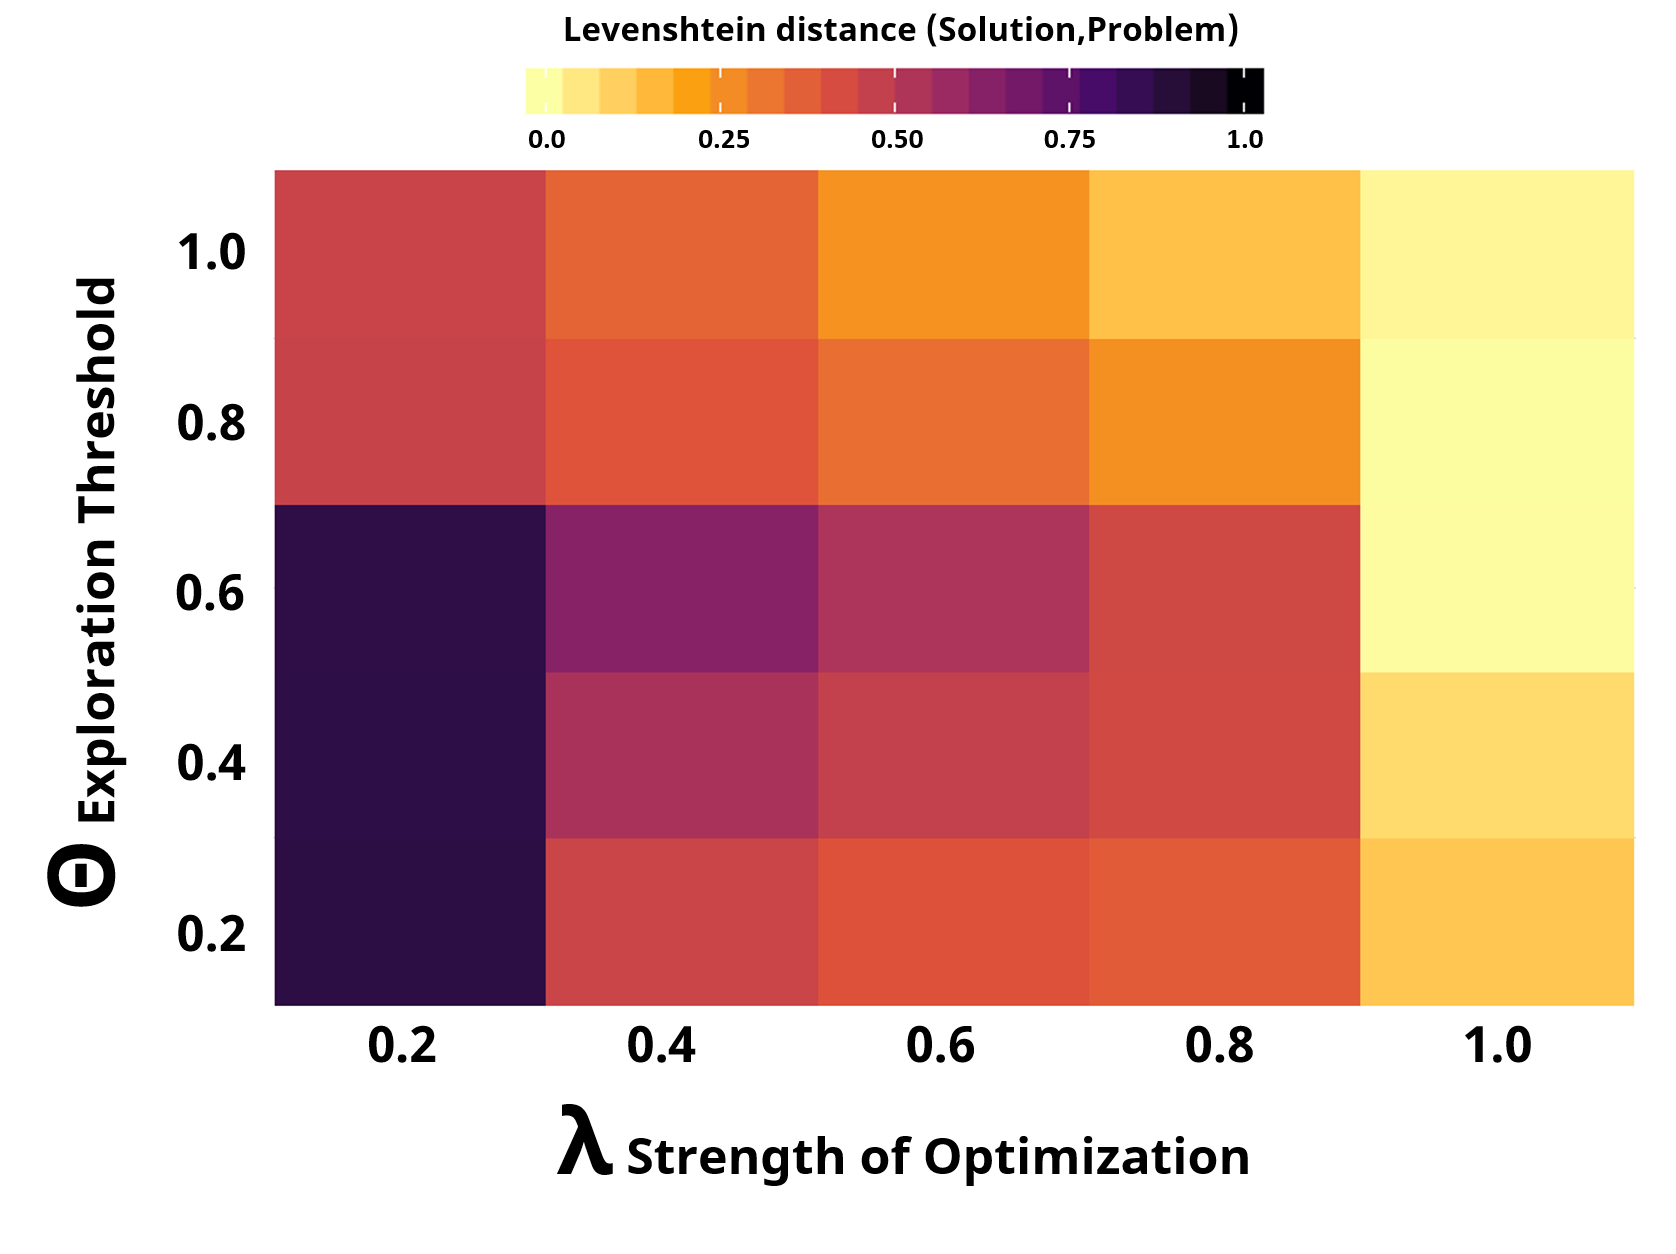
\includegraphics[width=\linewidth]{LD_heat.png}
    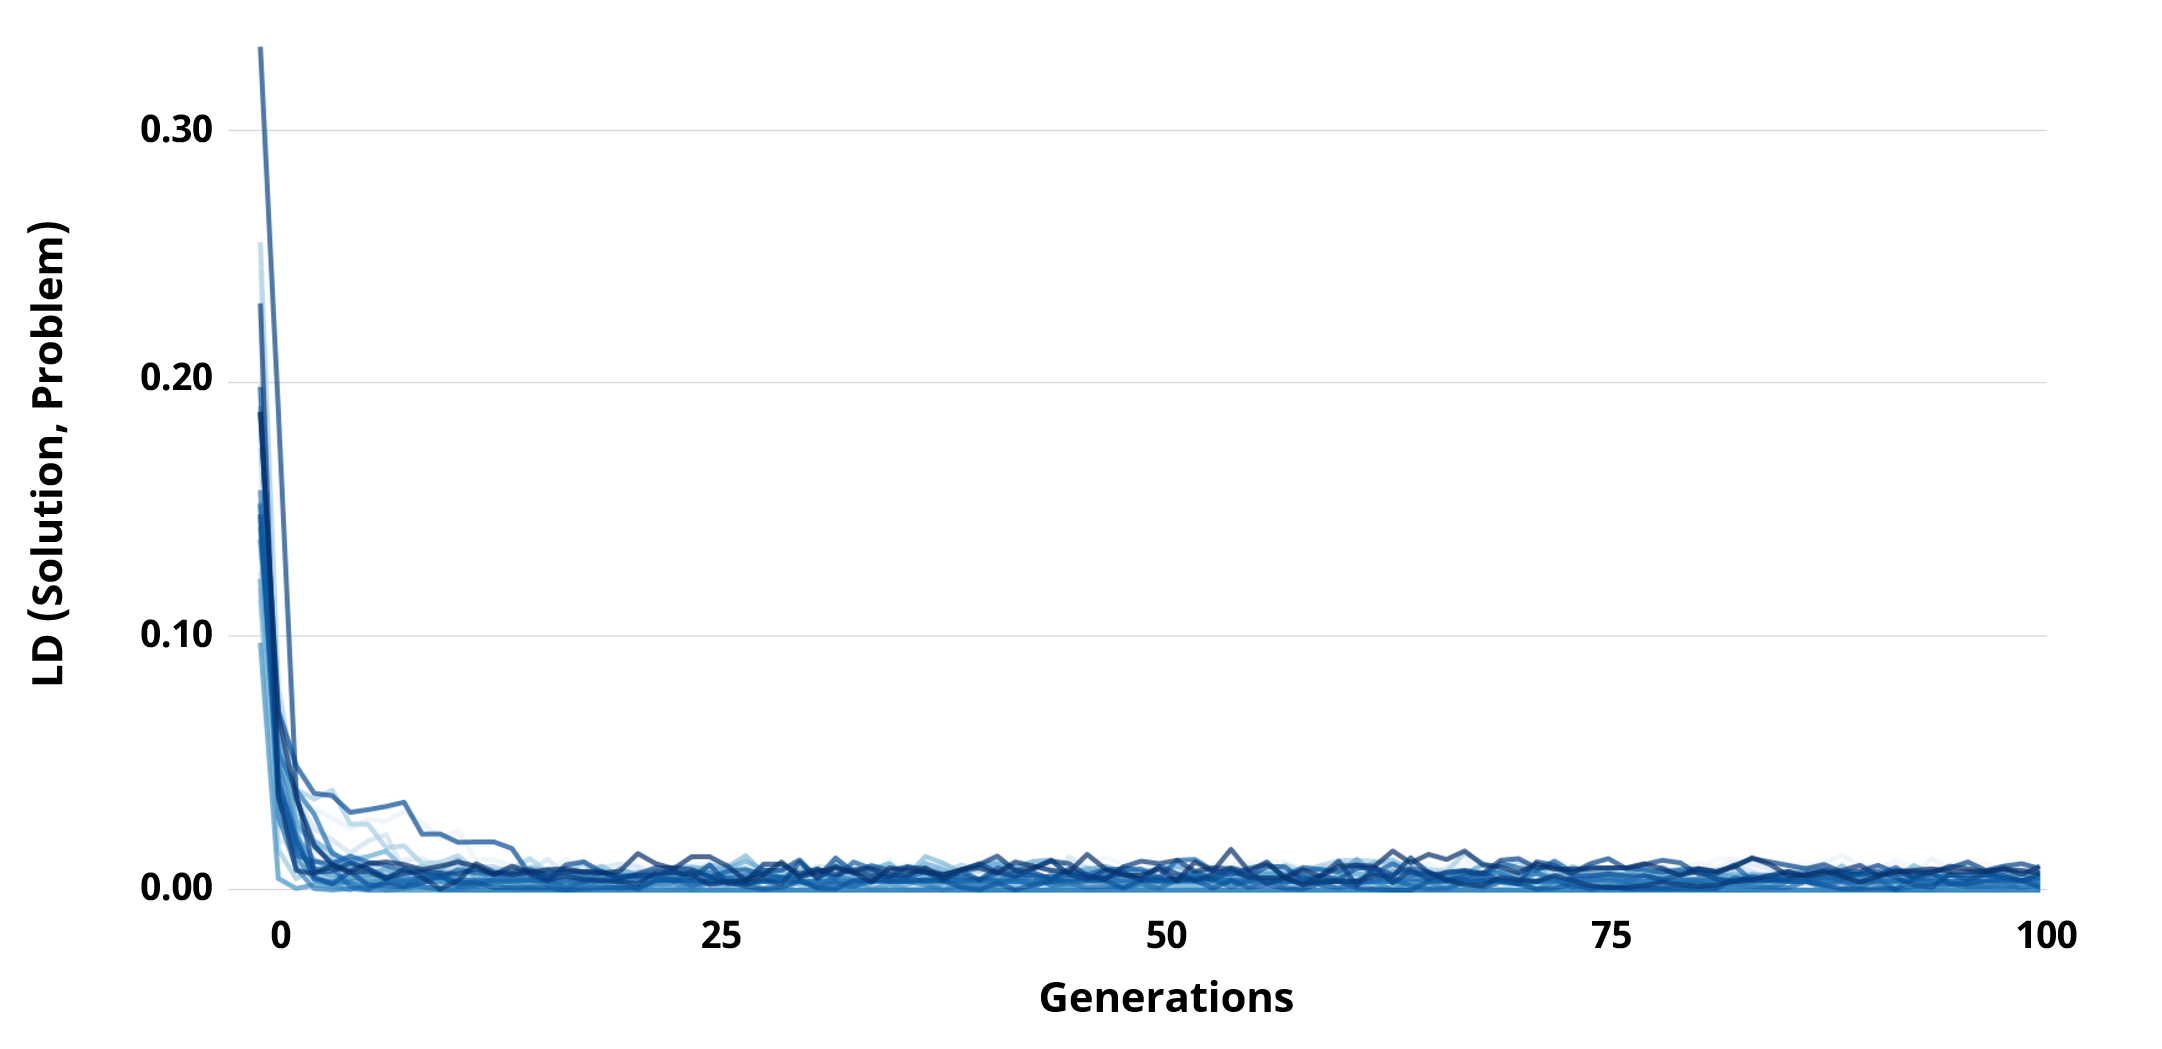
\includegraphics[width=\linewidth]{LD_runs.png}
\end{center}
    \caption{\textbf{Top:} Heatmap showing the average level of optimization at Generation~$=100$. Cells represent a specific parameter combination of $\lambda$ and $\Theta$ and colours corresponds to the (normalised) Levenshtein distance. Lighter colours denote solution-problem mappings with a lower Levenshtein distance. The x-axis is the strength of optimization ($\lambda$) and the y-axis is the range of exploration thresholds ($\Theta$).~\textbf{Bottom:} The average (normalised) Levenshtein distance of solution-problem mappings for a maximum optimization strength ($\lambda=1.0$) and an exploration threshold of $\Theta=0.4$. Coloured lines correspond to single runs over a $100$ generations ($1,000$ time-steps).}
    \label{fig:LD}
\end{figure}

Two factors sufficiently slow the exploration process to trap agents in these optimization cul-de-sacs. First, the topology of the problem space means that agents start out solving simpler input problems, which makes it easier for populations to converge on efficient fits. Second, if the exploration threshold is high (e.g., $\Theta=0.8$) and optimization is strong (e.g., $\lambda=1.0$), then the slow exploration of the problem space provides a stable enough target for optimization. Both the simplicity and stability of the input problem increase the probability of agents finding solutions below the exploration threshold: simpler input problems are computationally more tractable and stable problems provide more opportunities for agents to discover optimized solutions.

\begin{figure}[H]
\begin{center}
    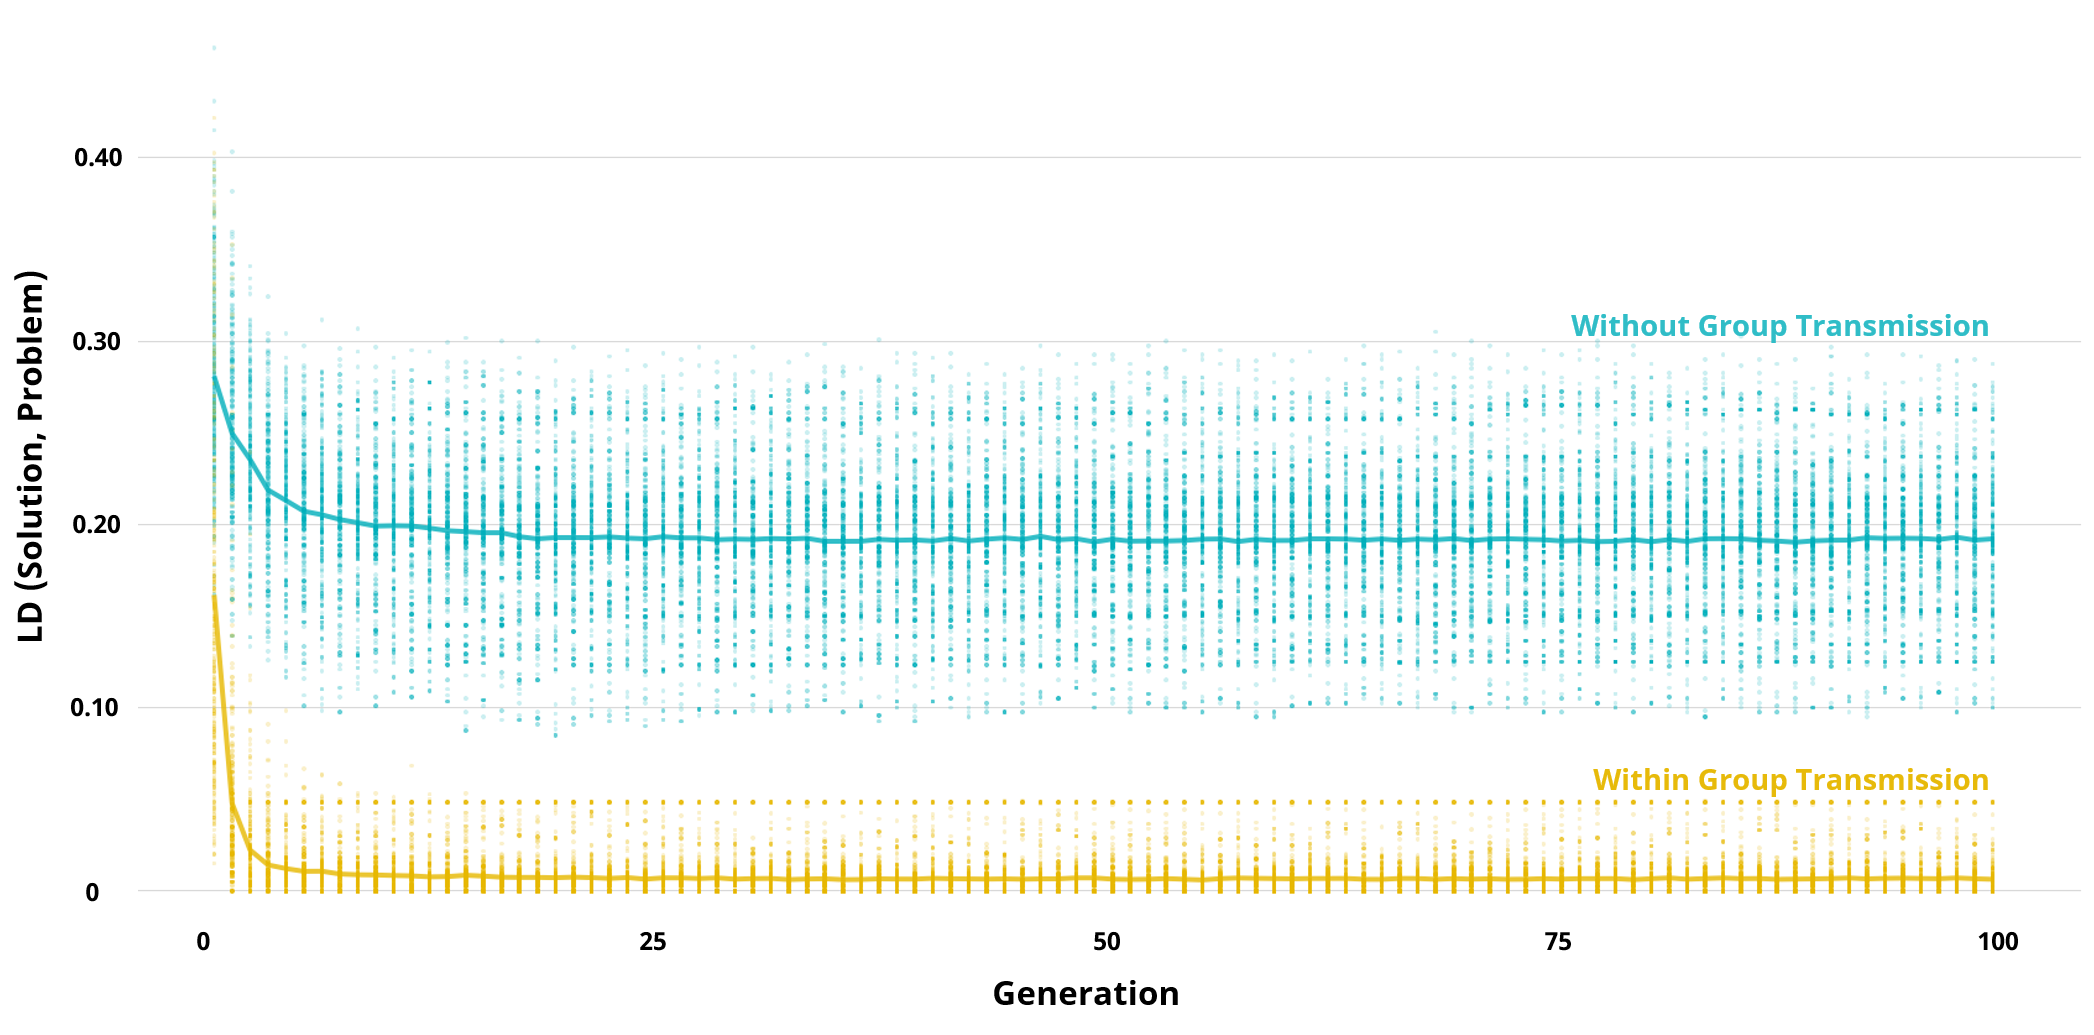
\includegraphics[width=\linewidth]{LD_optimal.png}
\end{center}
    \caption{Comparing runs with (gold) and without (turquoise) group transmission over $100$ generations when $\lambda=1.0$ and $\Theta=0.6$. Lines correspond to the average (normalized) Levenshtein distance and dots represent individual runs at a given generation.}
    \label{fig:LD_opt}
\end{figure}

A key question concerns the extent to which collective dynamics amplify this optimization process. One possibility is that within group transmission simply accelerates the rate of convergence in a population. If so, we should expect populations without access to group transmission to eventually converge on similarly optimized solutions to those populations utilizing within group transmission. As Fig.~\ref{fig:LD_opt} shows, when within group transmission is removed the optimizing potential of cultural evolution is diminished: populations asymptotically converge on sub-optimal solutions. It seems that having access to the pool of collective solutions not only accelerates convergence, but also leverages the collective computational potential of a population to discover and disseminate more optimized solutions.

\subsection{Open-ended cumulative dynamics require increasingly high rates of exploration relative to the strength of optimization}
Escaping these optimization traps requires increasingly high rates of exploration relative to the strength of optimization. An example of this is shown in Fig.~\ref{fig:complex} where the strength of optimization is at $\lambda=0.6$ and the exploration threshold corresponds to $\Theta=0.2$. Having a low exploration threshold facilitates rapid exploration of the problem space and allows agents to avoid optimization traps. Whereas optimization processes increase the fit between a solution and its input problem, exploration creates a moving target for optimization by repeatedly seeking out novel problems. The result is a positive feedback loop where there is a concomitant growth in the diversity and complexity of solutions.

\begin{figure}[H]
\begin{center}
    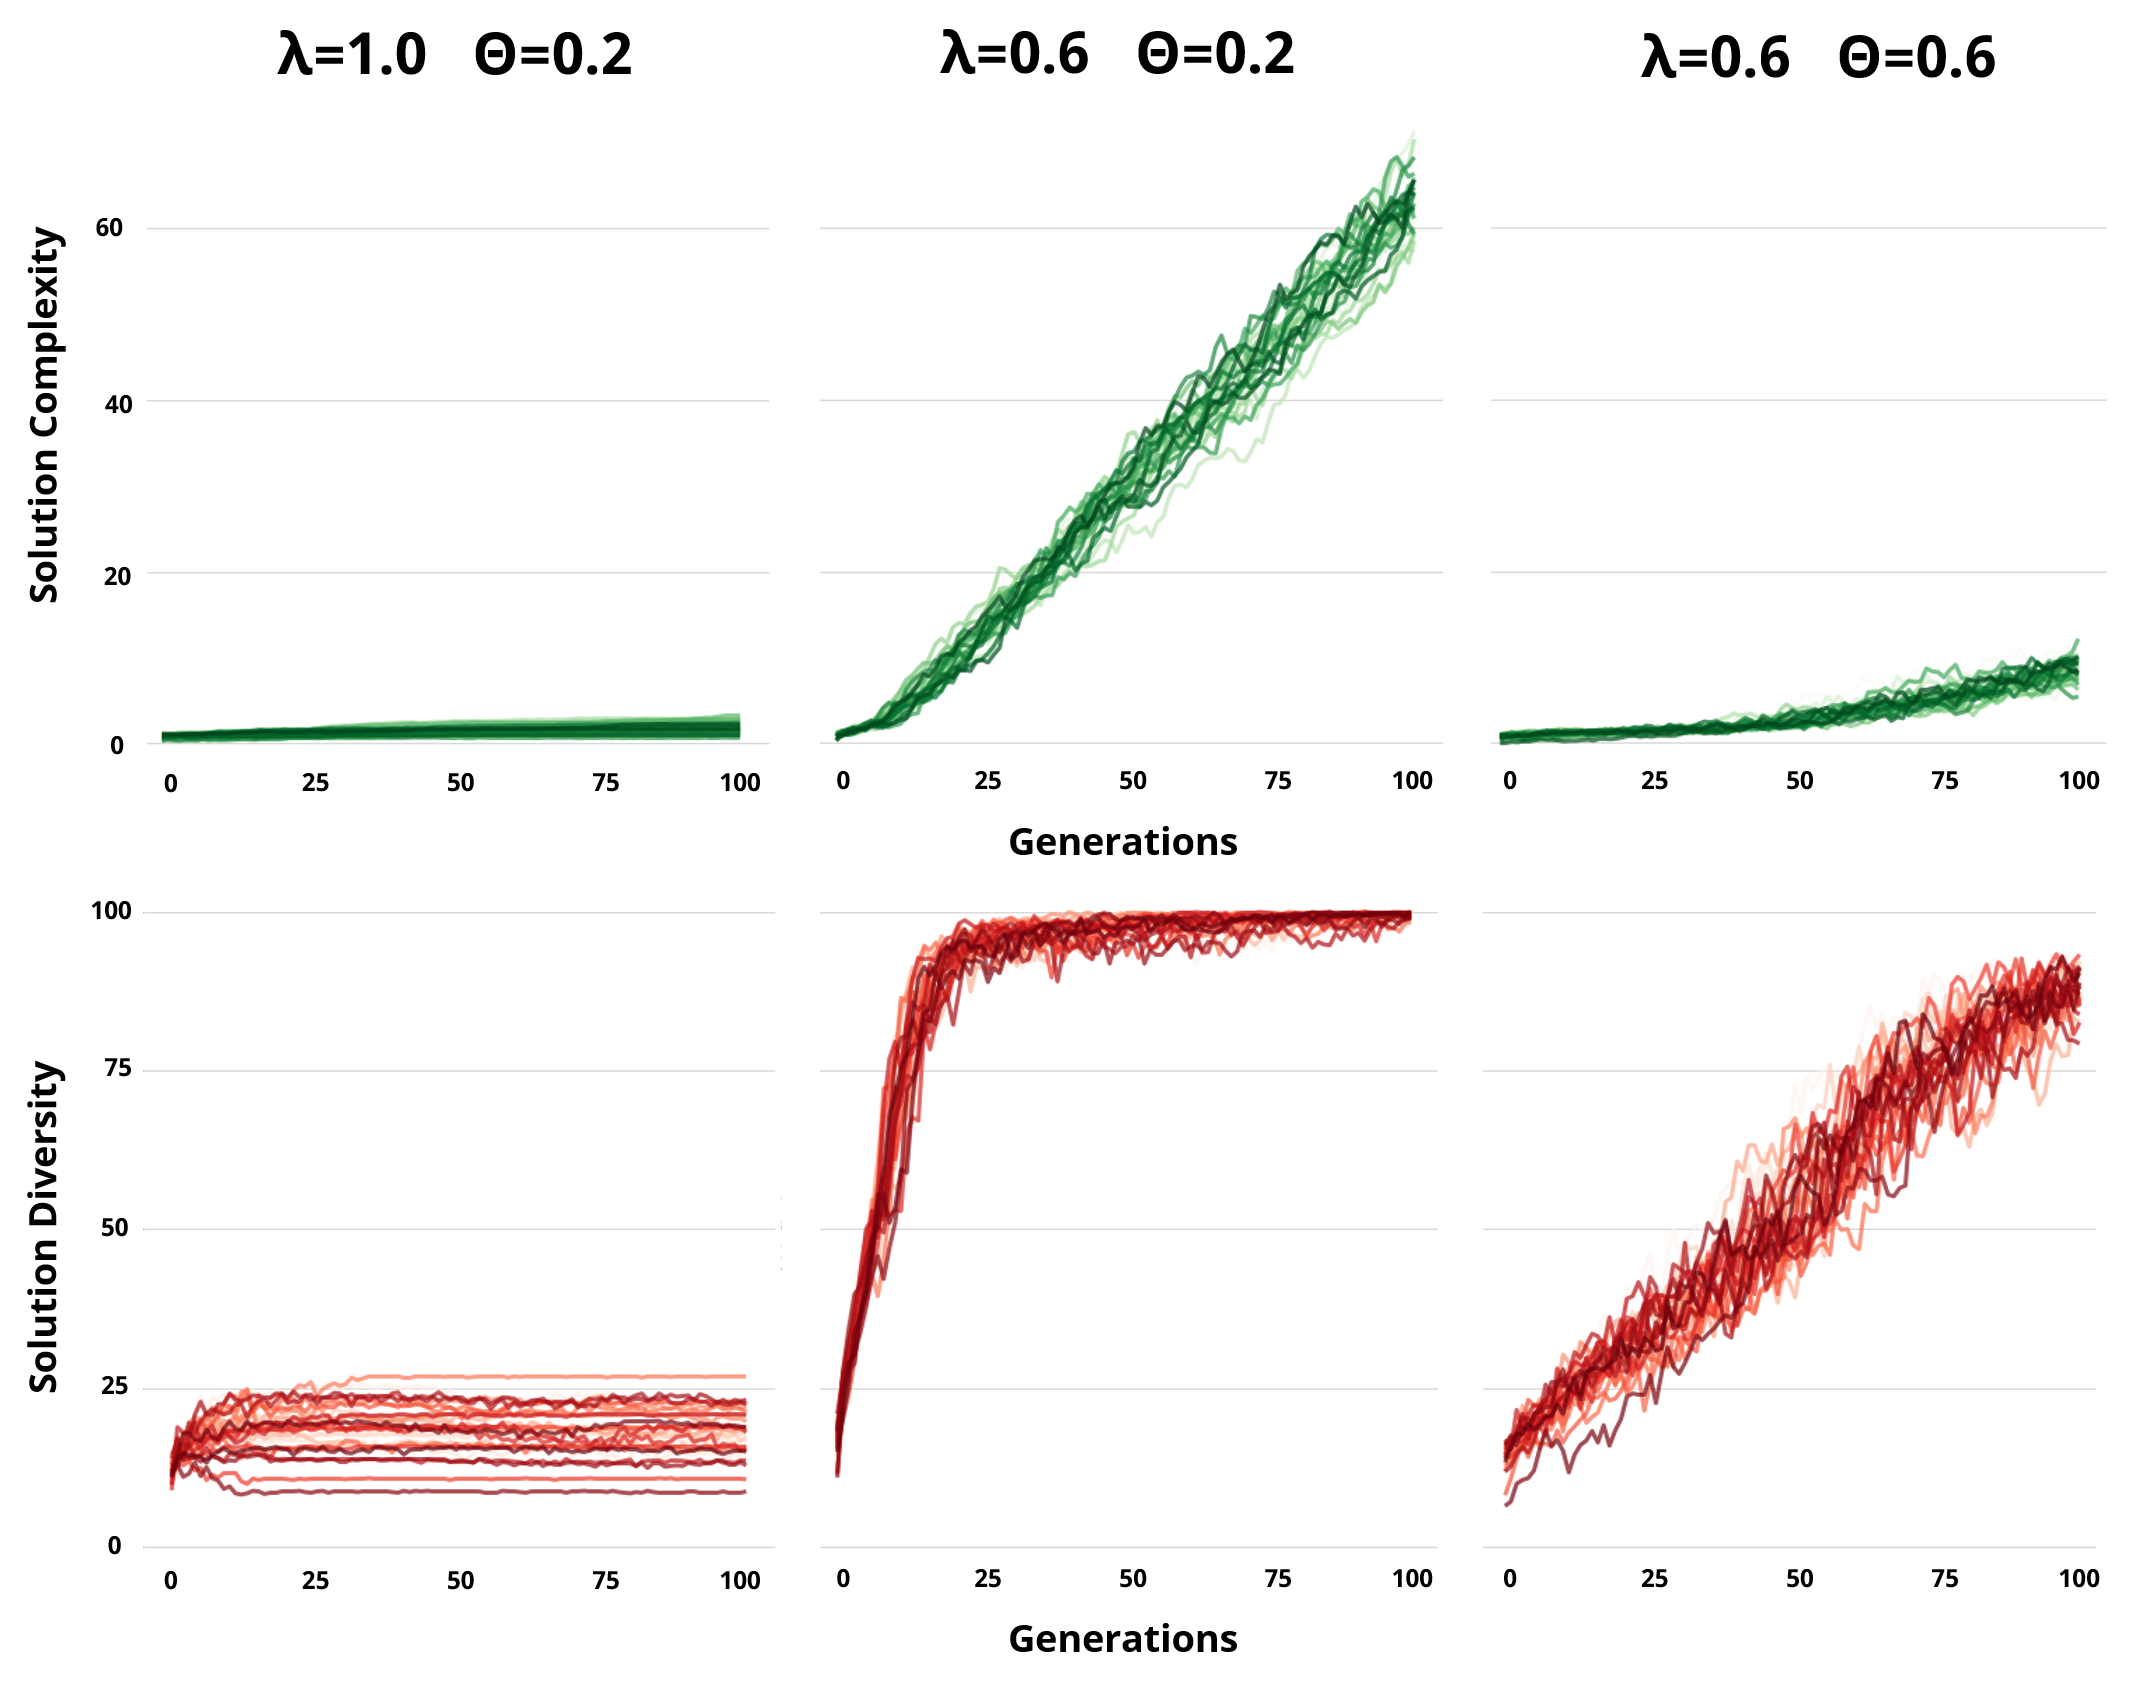
\includegraphics[width=\linewidth]{complexity.png}
\end{center}
    \caption{Time series of the average solution complexity (top row) and the average solution diversity (bottom row) for a $100$ generations. Solution complexity refers to $H_{L}(S)$ and solution diversity is the number of unique solutions in a population $s \in S$. As the population is fixed ($N=100$), there exists an upper bound on the total number of unique solutions a population can entertain. Each graph corresponds to a batch of 30 runs (coloured lines) for a specific parameter combination of $\lambda$ and $\Theta$. \textbf{Middle:} Outcomes where the strength of optimization is at $\lambda=0.6$ and the exploration threshold is at $\Theta=0.2$ result in open-ended cumulative culture. \textbf{Left:} If the strength of optimization is increased ($\lambda=1.0$), then the exploration threshold ($\Theta=0.2$) is insufficient for open-ended cumulative culture to emerge. \textbf{Right:} Lowering the strength of optimization ($\lambda=0.6$) and increasing the exploration threshold ($\Theta=0.2$) results in slower growth for both solution complexity and diversity.}
    \label{fig:complex}
\end{figure}

Increases in solution complexity reflect a general tendency towards solution strings that are longer and more entropic, whereas increases in diversity tells us that successive generations are host to more unique solution strings. Considering both measures together suggests that populations settle into a division of labour where growth is driven by agents exploring a wider range of increasingly difficult input problems. Harder input problems tend to be longer and less predictable and the probability of encountering such problems grows with $\ell(p)$. The intractability of harder input problems places a hard (computational) constraint on the extent to which populations can optimize and inhibits individual agents from dipping below low exploration thresholds.

Optimization must therefore be strong enough to keep apace with the difficulty of the input problem, but not so strong that populations end up in an optimization trap. As Fig.~\ref{fig:complex} shows, when optimization strength is increased ($\lambda=1.0$) relative to exploration ($\Theta=0.2$), the process of optimization dominates the amplification dynamics and is sufficient to stop open-ended cumulative culture from emerging. Relaxing the strength of optimization ($\lambda=0.6$) allows stochastic factors to play a role. With the rate of optimization slowed, amplification dynamics lead to an initial growth in diversity and complexity, which facilitates open-ended cumulative dynamics. However, if the exploration threshold is too high ($\Theta=0.6$), then growth in diversity is slowed and the complexity of solutions eventually stagnates in the long run.

\subsection{Social transmission plays an increasingly prominent role in maintaining open-ended cumulative dynamics}
Optimization alone is not sufficient to fully explain why we observe open-ended cumulative dynamics in some parameter combinations and not others. To understand why we need to also consider the contributions of different individual-level mechanisms. Previous theoretical and empirical studies have argued that open-ended cumulative culture requires asocial mechanisms for generating variation and social mechanisms for transmitting variation. The results here build on this by specifically delineating the contributions of these mechanisms in facilitating as well as maintaining cumulative culture.

Fig.~\ref{fig:event} shows the aetiology of solutions for the same three parameter combinations as in the previous section. Runs where open-ended cumulative culture ($\lambda=0.6$; $\Theta=0.2$) emerges show a distinct dynamic to situations where solutions are either highly optimized ($\lambda=1.0$; $\Theta=0.2$) or are bounded at a certain level of complexity ($\lambda=0.6$; $\Theta=0.6$). Initially, asocial mechanisms are necessary and sufficient to bridge the gap between problem difficulty and solution complexity, with invention and modification providing the main contributions to the emergence of open-ended cumulative culture.

\begin{figure}[H]
\begin{center}
    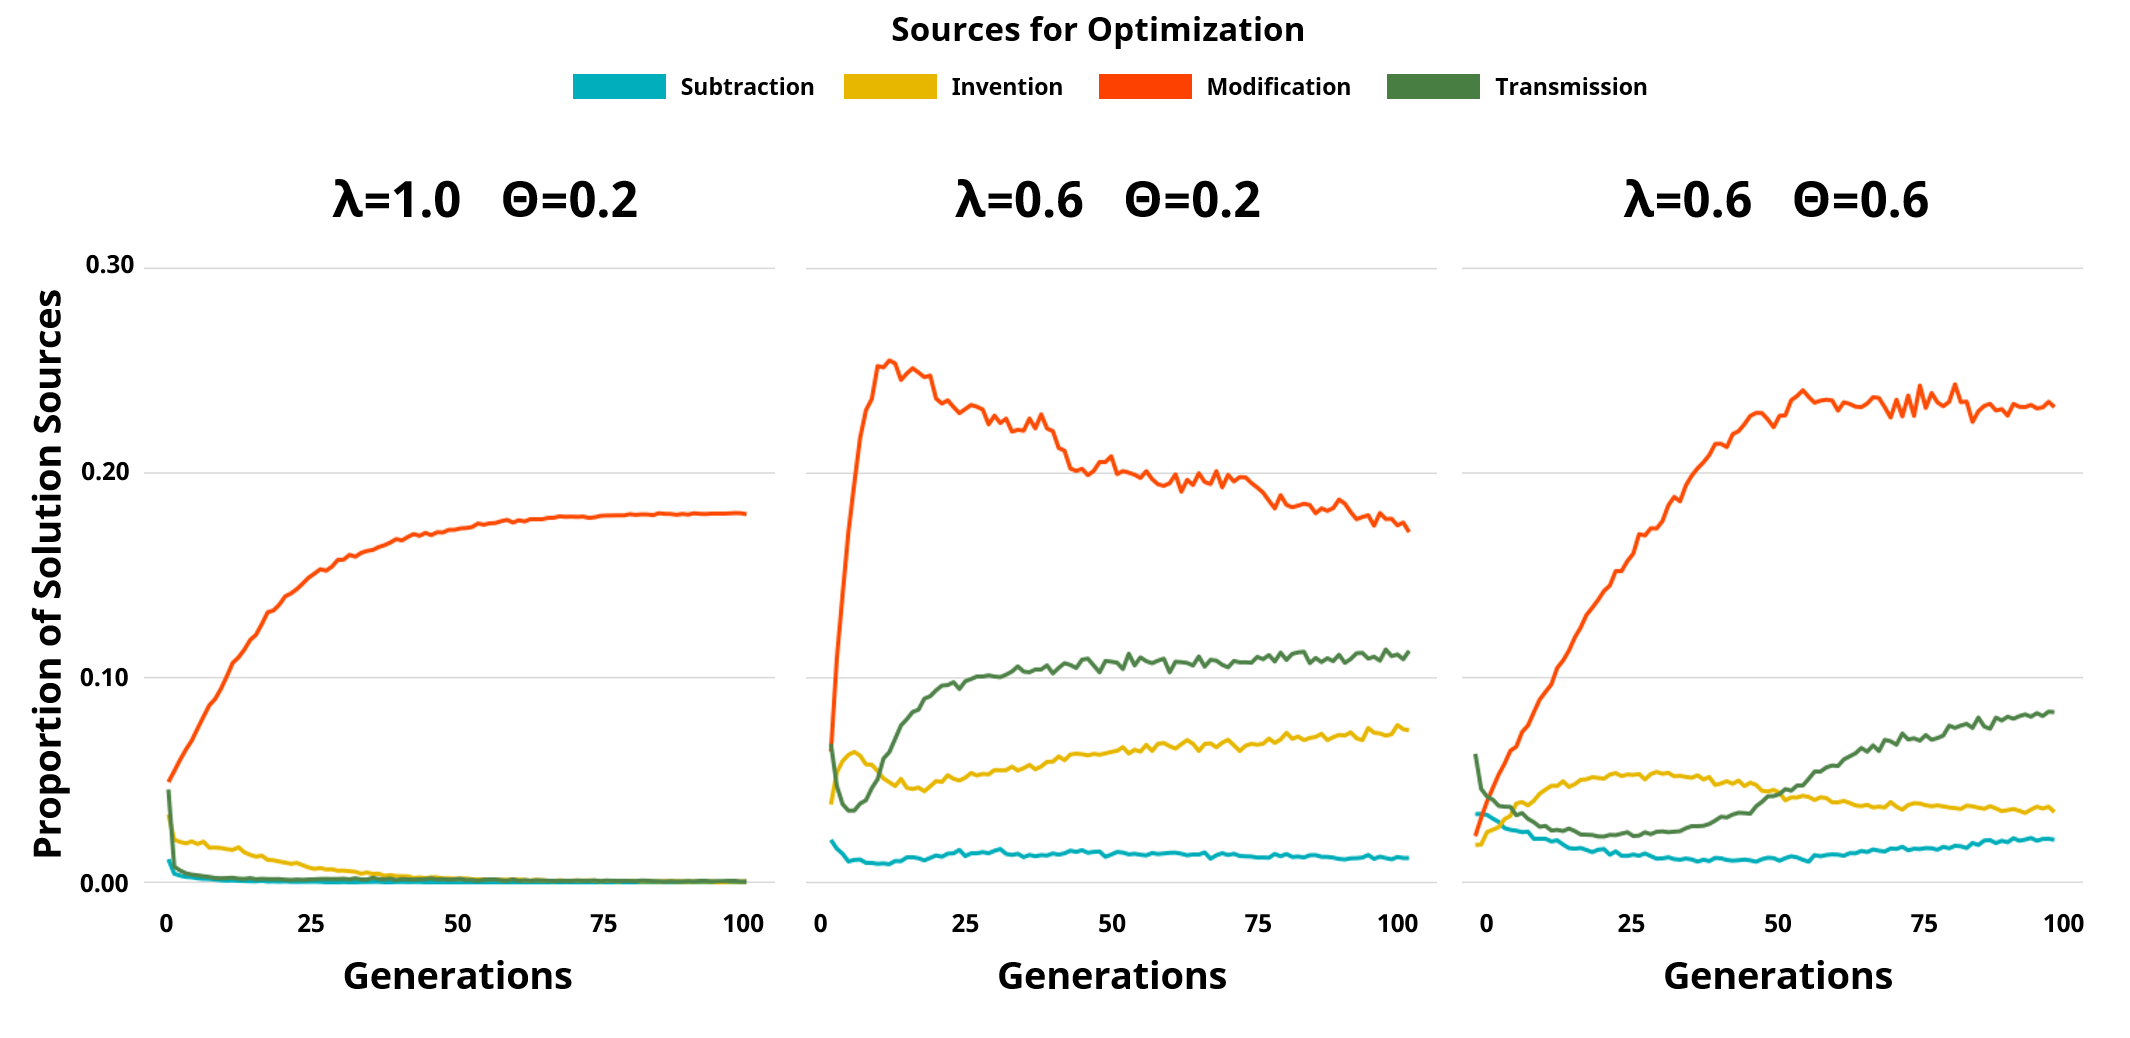
\includegraphics[width=\linewidth]{choices.png}
\end{center}
    \caption{Average selection probability of solutions from social and asocial sources over $100$ generations. Coloured lines represent the specific social or asocial source. \textbf{Middle:} Proportion of chosen solutions when strength of optimization is at $\lambda=0.6$ and the exploration threshold corresponds to $\Theta=0.2$ (resulting in open-ended cumulative culture). \textbf{Left:} Proportion of chosen solutions when the strength of optimization is at $\lambda=1.0$ and the exploration threshold is $\Theta=0.2$ (resulting in highly optimized cultures). \textbf{Right:} Proportion of chosen solutions when the strength of optimization is at $\lambda=0.6$ and the exploration threshold is $\Theta=0.6$ (resulting in cultures where complexity stagnates).}
    \label{fig:event}
\end{figure}

However, following this initial phase of growth, optimization increasingly relies on within-group transmission dynamics. Within-group social transmission allows a population to leverage its collective computational potential and bypass individual limitations in searching the space of possible solutions. Innovations by one individual can be disseminated to others in a population far quicker than an individual independently arriving at an equivalent solution. This benefit is particularly apparent when optimization needs to keep apace with increasingly difficult input problems: unbounded growth in complexity is only maintained when a significant proportion of solutions are transmitted between agents. 

To test this assumption, with fixed optimization ($\lambda=0.6$) and exploration ($\Theta=0.2$) parameters, an additional simulation was run where within-group transmission was removed as a mechanism. When compared to simulation runs where within-group transmission is present (see Fig.~\ref{fig:transmission}), the levels of complexity are far lower in runs for agents who solely rely on asocial generative mechanisms. What this tells us is that the potential of asocial mechanisms is fundamentally capped at a certain level of solution complexity. Overcoming this upper bound on complexity requires within-group social transmission.

\begin{figure}[H]
\begin{center}
    \includegraphics[width=\linewidth]{transmission.png}
\end{center}
    \caption{Solution complexity over $100$ generations when $\lambda=0.6$ and $\Theta=0.2$ for runs with (gold) and without (turquoise) group transmission. Lines correspond to the average level of solution complexity and dots represent individual runs at a given generation.}
    \label{fig:transmission}
\end{figure}

\section{Discussion}
Two general processes are usually invoked as explanatory concepts of technological evolution: the first is an optimizing process where technologies are refined towards a functional objective ({\em cultural adaptation}) and the second re-purposes existing technologies towards a new functional goal ({\em cultural exaptation}). The current paper modelled cultural adaptation as an optimizing search over a solution space and cultural exaptation as a local search over the space of possible problems. By manipulating two general parameters, corresponding to the strength of optimization ($\lambda$) and an exploration threshold ($\Theta$), this model helps delineate the contributions of these processes to cultural evolutionary dynamics. In particular, this paper showed that:

\begin{enumerate}[(i)]
    \item Cultural dynamics often lead to optimization traps when the strength of optimization is strong relative to the rate of exploration;
    \item Escaping these optimization traps relies on a feedback loop between exploration and optimization that results in a concomitant growth in the complexity and diversity of solutions;
    \item This initial emergence of open-ended cumulative culture is reliant on asocial generative mechanisms of innovation;
    \item But maintaining these open-ended dynamics increasingly requires social transmission.
\end{enumerate}

\subsection{Optimization traps and the strength of optimization ($\lambda$)}
Cultural evolutionary dynamics are often envisaged as an optimization process~\cite{xxxx}. The results here build on the existing literature by clearly delineating where cumulative dynamics lead to open-ended growth in complexity and where populations end up in optimization traps. Generally, when the strength of optimization is at maximum ($\lambda=1.0$), and the collection of input problems form a stable target, populations are able to reach highly optimized solutions. Having stable input problems increases the probability of populations dipping below the exploration threshold and limits any further exploration of the problem space.

Optimization traps might help explain why open-ended cumulative culture is rare in nature. If populations are restricted to a limited set of stable input problems, and populations have high levels of within-group transmission, then strong optimization pressures will inhibit exploration of novel problems and trap cultures in local regions of the solution space. Such insights complement existing explanations for periods of relative stasis~\cite{powell2009late} or reversals~\cite{henrich2004demography} in the technological complexity of toolkits during human pre-history. It also mirrors, in some respect, what we observe in social transmission experiments~\cite{xxxx}: a stable target and a cultural evolutionary process will tend to converge on highly optimized outcomes.

Within-group transmission acts a strong amplifier on optimization: optimal solutions more rapidly disseminate between individuals, drastically reducing the search load on asocial mechanisms (and inheritance). In the absence of within-group transmission, the optimizing potential of cultural evolution is greatly diminished, with populations tending to stabilize around sub-optimal solutions. This suggests high levels of within-group transmission act as a barrier to the emergence of open-ended cumulative culture. Further work is required to establish whether this finding generalises to empirical findings. However, if accurate, we are left with a curious conundrum: within-group transmission needs to be inhibited for open-ended cumulative culture to emerge, but it is central to maintaining these dynamics over long timescales. 

\subsection{Open-ended cumulative culture and the exploration threshold ($\Theta$)}
Relaxing the strength of optimization allows populations to escape optimization traps by facilitating growth in both the diversity and complexity of solutions. Reaching open-ended cumulative culture also requires increasingly high rates of exploration. Motivating this search over the problem space is the extent to which solutions are already optimized. Lower thresholds generally correspond to increased rates of exploration as agents are continually seeking out new opportunities for repurposing. Importantly, for open-ended cumulative culture to emerge, optimization dynamics must be able to chase this movement through the problem space.

Maintaining this dynamic requires the exploration threshold is low enough to discover harder input problems and create a pressure for more complex solutions. The topology of the problem space plays an outsized role in this process. In particular, harder input problems place greater constraints on the potential for optimization. Having a sufficiently low exploration threshold, as well as an increased probability of encountering harder input problems, results in an exploration rate that is quick enough to slow down the optimization process and stops populations from becoming trapped in certain regions of the problem space. Crucially, these findings come from separating out the search processes over solution and problem spaces. Doing so also allowed us to more readily classify problems based on their difficulty and recognises that finding an optimal solution is intractable for certain classes of problem. Characterising the dynamics of culture in terms of computation also raises an important yet rarely appreciated point: that the properties of a given input problem can act as a constraint independently of specific cognitive, ecological, or culturally endogenous factors.

One general hypothesis that follows from this is that cultural exaptation is driven by differences in the level at which solutions are optimized. This predicts that highly optimized solutions resist repurposing and lead to optimization traps. Why might highly optimized solutions have a lower repurposing potential than suboptimal ones? One possibility, which is considered here, is that optimization can be likened to overfitting in statistical models. Relative to optimized solutions, which are finely tailored to their input problem, suboptimal solutions have a latent potential for finding a range of more appropriate fits. Optimized solutions, by contrast, are less generalisable to novel problems due to a high degree of specialization: any movement to a new problem has a high probability of significantly reducing the fit.

Case studies of technological exaptation note that repurposing is sometimes correlated with limitations in a solution's existing functional role~\cite{arthur2009nature}. Today, the main use of cavity magnetrons is in microwave ovens, but originally they were a vital component of radar technology. Yet, even in their heyday, a well-documented limitation of radar-driven magnetrons was an inability to easily remove clutter on displays~\cite{brookner201010}. Eventually, this led to magnetrons being replaced in radar by more suitable alternatives. Still, it remains an open question as to whether or not some technologies differ in their underlying capacity to be repurposed, and more empirical work is needed to establish if the potential of cultural exaptation is linked to the degree of optimization.

\subsection{Asocial and Social mechanisms in the emergence and maintenance of open-ended cumulative culture}
Considerable debate exists over the underlying capacities for cumulative culture and the respective roles individual creativity and social transmission~\cite{xxxtomasello,enquist2011modelling,lewis2012transmission,charbonneau_all_2015,zwirner2015cognitive}. The findings here suggest that asocial mechanisms of innovation (specifically {\em invention} and {\em modification}) are generally more important than within-group transmission in the emergence of cumulative culture. However, asocial mechanisms are insufficient to maintain open-ended growth past a certain level of solution complexity. Once individuals reach this complexity ceiling, differences between the input problem and the current solution are large enough that most single-edit changes fail to improve the fit, and agents will instead choose to remain with their current solution.

By distinguishing between the emergence and maintenance of open-ended cumulative culture, the model here presents a more nuanced role for both within-group transmission and asocial mechanisms for generating variation. Initially, within-group transmission plays a marginal role in the emergence of open-ended cumulative culture, with solutions from asocial sources providing the principle gains in diversity and complexity. Besides the inherent advantages of asocial sources, socially transmitted solutions are disadvantaged at this early stage for two reasons. First, at the individual-level, the reconstructive nature of learning means that solutions are prone to information loss, which was modelled here as a bias for efficient representations. Second, the adoption of socially transmitted solutions generally promotes convergence at a population-level, resulting in a homogenising process where diversity is lost and searches are confined to local regions of the solution space.

Only when populations are faced with diverse and increasingly difficult problems are the benefits of within-group social transmission unmasked. By rapidly spreading solutions between individuals, transmission stops individual agents from becoming trapped in local regions of the solution space, and provides populations with the opportunity to breach the complexity ceiling faced by solutions from asocial sources. Such benefits cannot be understated: populations become increasingly reliant on within-group transmission even though the process is biased against complexity. Part of the rationale for this is that the upside of convergence is enough to mitigate the simplifying effects of information loss. All that is required is for transmission to raise the average level of complexity enough for asocial mechanisms and optimization to keep apace with the high rates of exploration.

\subsection{Assumptions}
Examining the assumptions of this model is important for future work to critically assess and empirically test the robustness and generalisability of these claims. 

Optimization is conceptualized here as an individual-level decision-making process. One advantage of this approach is it provides us with a means of directly comparing the contributions of social and asocial mechanisms. A key assumption is that making a decision is solely focused on discovering a locally optimal solution. However, as documented in behavioural economics, there are many other factors at work in shaping the choice architecture of individuals. Furthermore, these biasing factors can act antagonistically to functional pressures. For instance, in the now almost-forgotten format war over the de facto video cassette standard, the success of VHS over the technically superior Betamax was driven by economic and social factors.

A second assumption concerns the constraints on innovation and transmission. Nearly all models of cognition introduce some means of transformation on the way agents produces and process information. Innovation mechanisms were assumed to be incremental and derivative: individual agents can only perform single-edit changes to existing solutions. The goal here was to approximate limitations on innovation by restricting trial and error tinkering to local regions of the solution space. Of course, it is often the case that innovations are not constrained to incremental searches, and instead make large jumps via revelatory insights~\cite{villani2007agent} or recombination~\cite{charbonneau2016modularity}. Social transmission, on the other hand, was biased towards parsimonious representations of solutions. This links with prominent and strongly supported models both in cognitive science~\cite{xxxx} and cultural evolution~\cite{xxxx}, but it is possible that reconstruction is not always biased in the direction of simplicity~\cite{xxxx}.

The third major assumption is that the population dynamics were relatively impoverished. The process of within-group transmission was determined by randomly sampling a single solution of another agent from the population. Restricting the pool of solutions meant that a single agent only samples a small proportion of the total culture at any given time step. Furthermore, there was no consideration of population growth, and agents did not take into account non-functional information when sampling from individuals (e.g., social status). Yet, we know that the network topology of human populations are not randomly connected graphs~\cite{albert2002statistical}, population size is not a static feature~\cite{creanza2017greater}, and the sampling of individuals and solutions is often socially biased (e.g., conformity~\cite{richerson_not_2008}). Alternative models of network structure, which incorporate growth (see Barab\'asi–Albert model~\cite{barabasi1999emergence}) and rewiring (see Watts and Strogatz model~\cite{watts1998collective}), provide potential avenues for future work to provide a richer link between individual-level processes and population-level dynamics.

Finally, several assumptions were made with respect to the exploration threshold, how the problem space was structured, and the way in which agents move between different input problems. For instance, there are several alternative ways the exploration threshold could have been approached. The simplest formulation is one where a parameter determines a fixed rate of movement. One issue with this specific formulation is that agents would move irrespective of whether a solution was perfectly or poorly optimized. Crucially, it precludes the possibility that populations can become trapped in regions of the space. Coupling the exploration process to optimization allows us to observe how different strengths of optimization interact with exploration in influencing cultural evolutionary dynamics. Nevertheless, it is likely that changes to the exploration threshold, as well as manipulations to the ability with which agents can traverse the problem space, are necessary steps for future work. 

\section{Conclusion}
Explaining the origins of cumulative culture, and how it is maintained over long timescales, constitutes a fundamental challenge for theories of cultural evolution. Previous theoretical work has emphasised two fundamental causal processes: cultural adaptation (where technologies are refined towards a functional objective) and cultural exaptation (the repurposing of existing technologies towards a new functional goal). Yet, despite the prominence of cultural exaptation in these theoretical explanations, this process is often absent from models and experiments investigating cumulative culture. Using an agent-based model, where agents attempt to solve problems in a high-dimensional problem space, this paper found that open-ended cumulative culture only emerges under a restricted set of parameters.

In many cases, cultural dynamics push populations into optimization traps: here, excessive optimization of solutions cause the dynamics of change to cease, with populations entering a state of equilibrium. Escaping these optimization traps requires cultural dynamics to explore the problem space rapidly enough to create a moving target for selection. This sets in motion a positive feedback loop where there is open-ended growth in the complexity of cultural solutions. Finally, the results helped delineate the roles played by social and asocial mechanisms, with asocial mechanisms of innovation driving the emergence of cumulative cultural evolution and social mechanisms of within-group transmission helping maintain these dynamics over long timescales.

\section*{Data Availability}
All code and data is available at the following GitHub repository:~\href{https://}{https://}

\section*{Competing Interests}
The authors declare no competing interests.

\section*{Acknowledgements}
The author would like to thank Olivier Morin and Oleg Sobchuk for helpful and insightful comments on earlier versions of this paper.

\bibliographystyle{unsrt}
\bibliography{lit}

\end{document}